\section{2018 Sun-Climate Symposium}

\frame
{
%...................................................................................................
\note<1>[item]{The Str\"omgren filters B and Y, as well as the Kepler passband or the COROT filter, are broadly used for observations.

Therefore, these filters are of particular interest when radiative transfer calculations are performed. Currently, this is computationally demanding due to a huge amount of atomic and molecular lines.

In this talk, I will show that a SIGNIFICANT speed up can be achieved by using optimized opacity detribution functions, which we call OODF!

Let’s start with the example of the Strömgren Y filter. As you can see the intensity is dominated by lines….}
%...................................................................................................
	\frametitle{Exemplary case of Str\"omgren \textit{y} filter}
	\begin{itemize}
		\item Complex structure of spectrum due to lines
	\end{itemize}
	\centering
	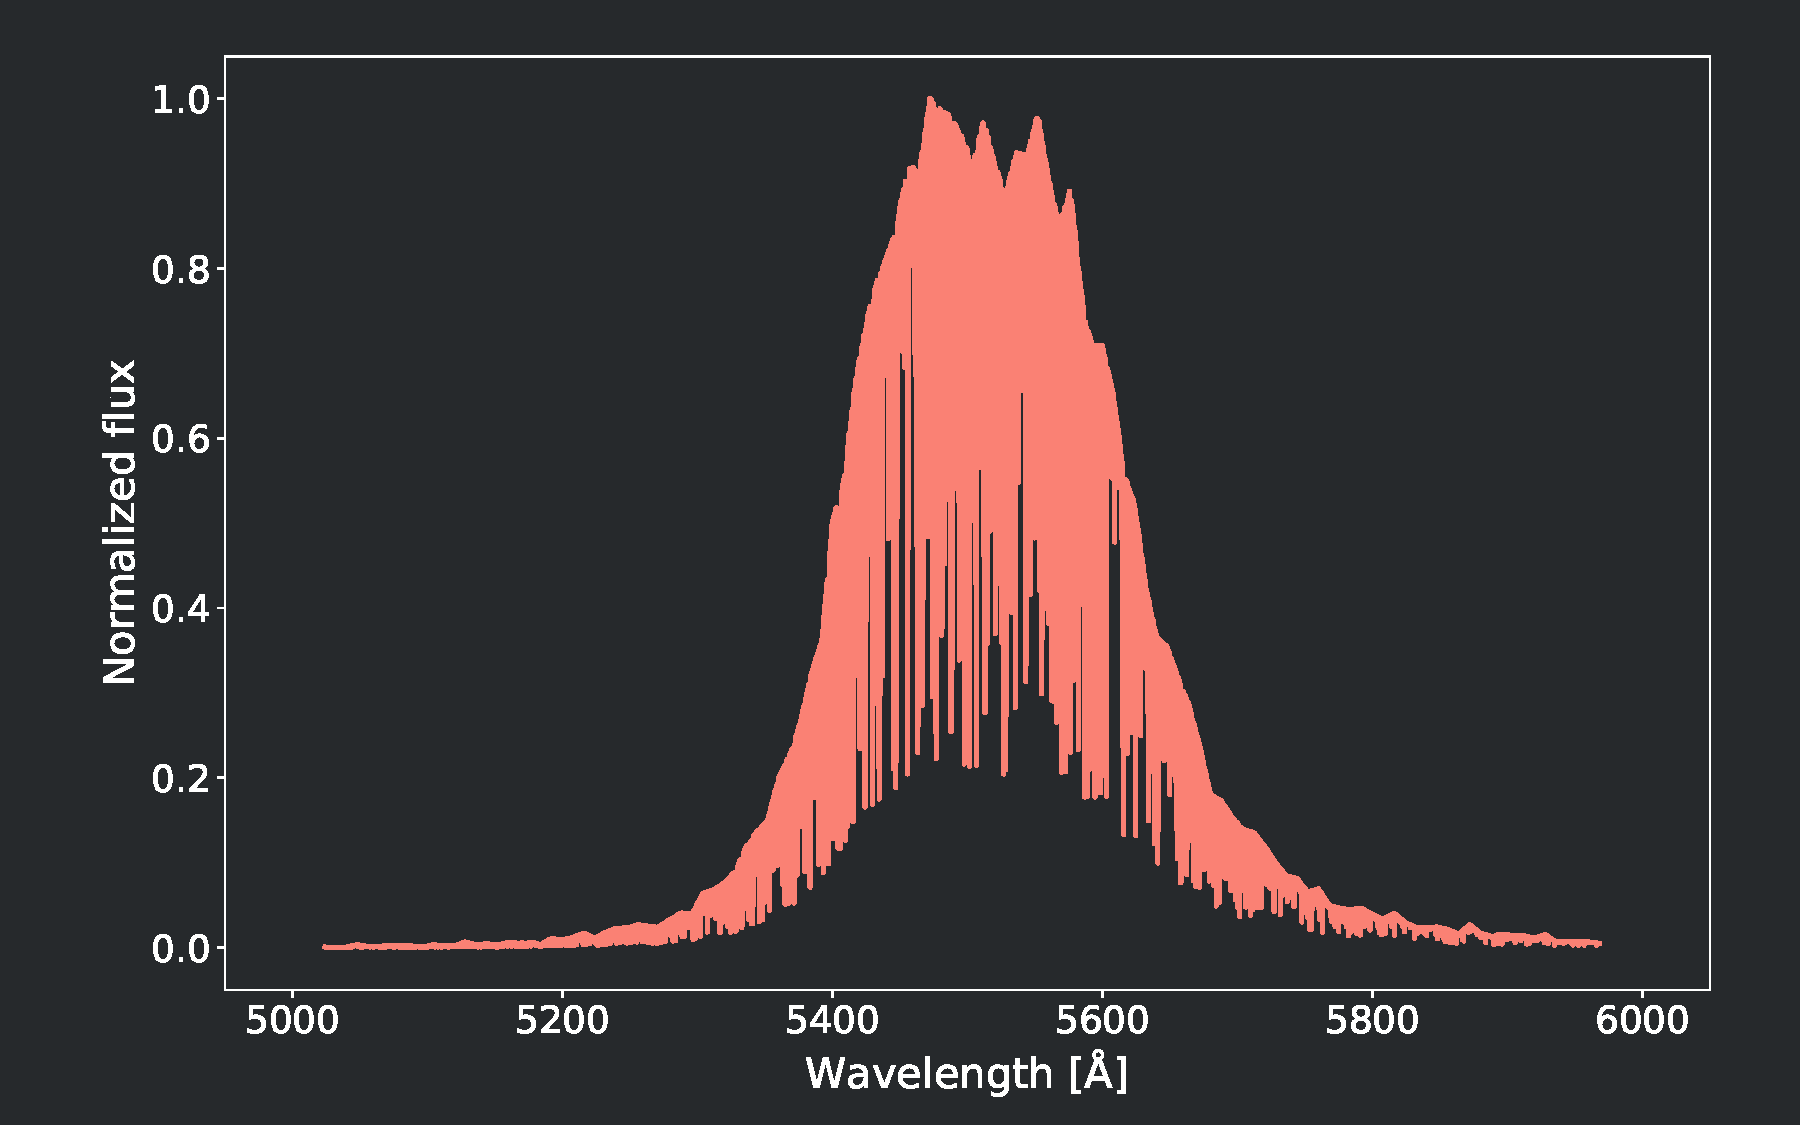
\includegraphics[width=115mm]{images/spectra_transmitted_and_opacity_0}
}
\frame
{
%...................................................................................................
\note<1>[item]{Take notes here.}
%...................................................................................................
	\frametitle{Complex structure of opacity}
	\begin{itemize}
		\item Opacity varies by multiple orders of magnitude within 1\si{\angstrom}
	\end{itemize}
	\centering
	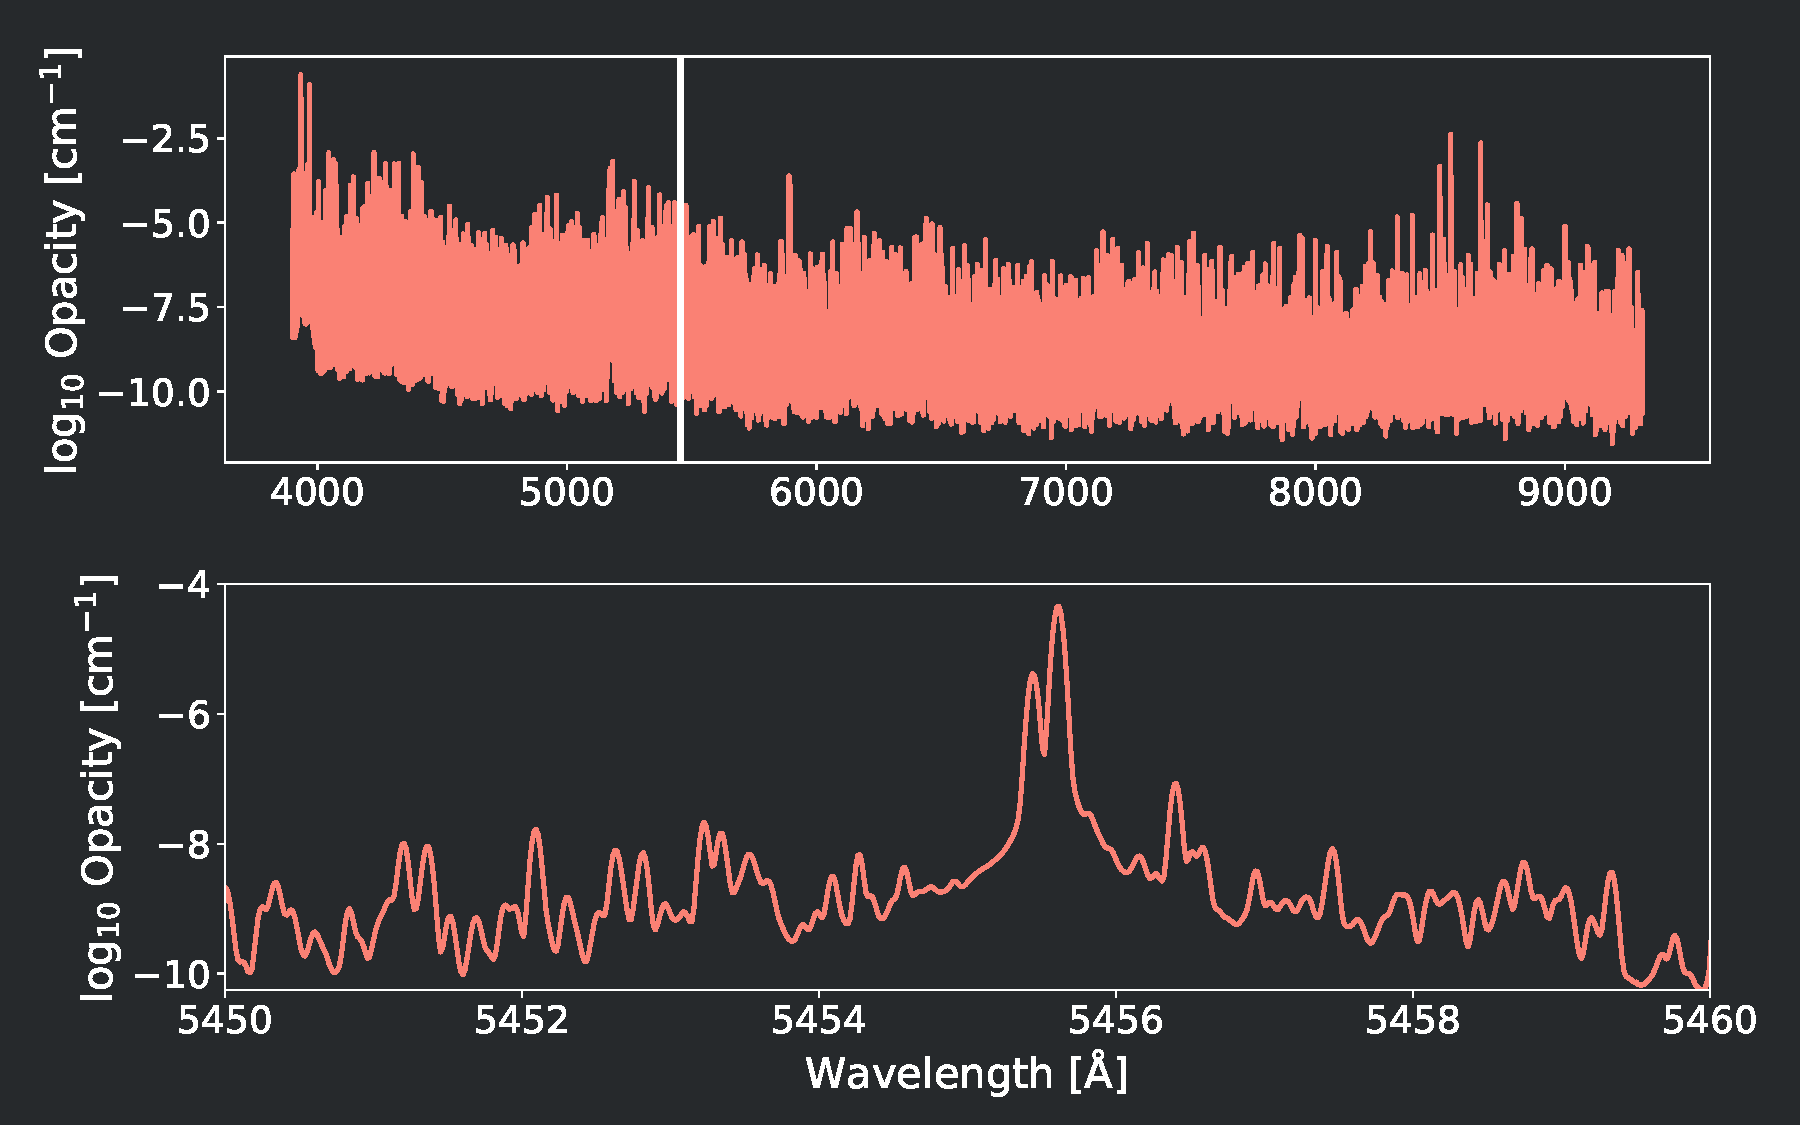
\includegraphics[width=115mm]{images/spectra_transmitted_and_opacity_1}
}

\frame
{
%...................................................................................................
\note<1>[item]{Take notes here.}
%...................................................................................................
	\frametitle{Sorting by opacity}
	\begin{itemize}
		\item Sort wavelength points by corresponding values of opacity
	\end{itemize}
    \centering
	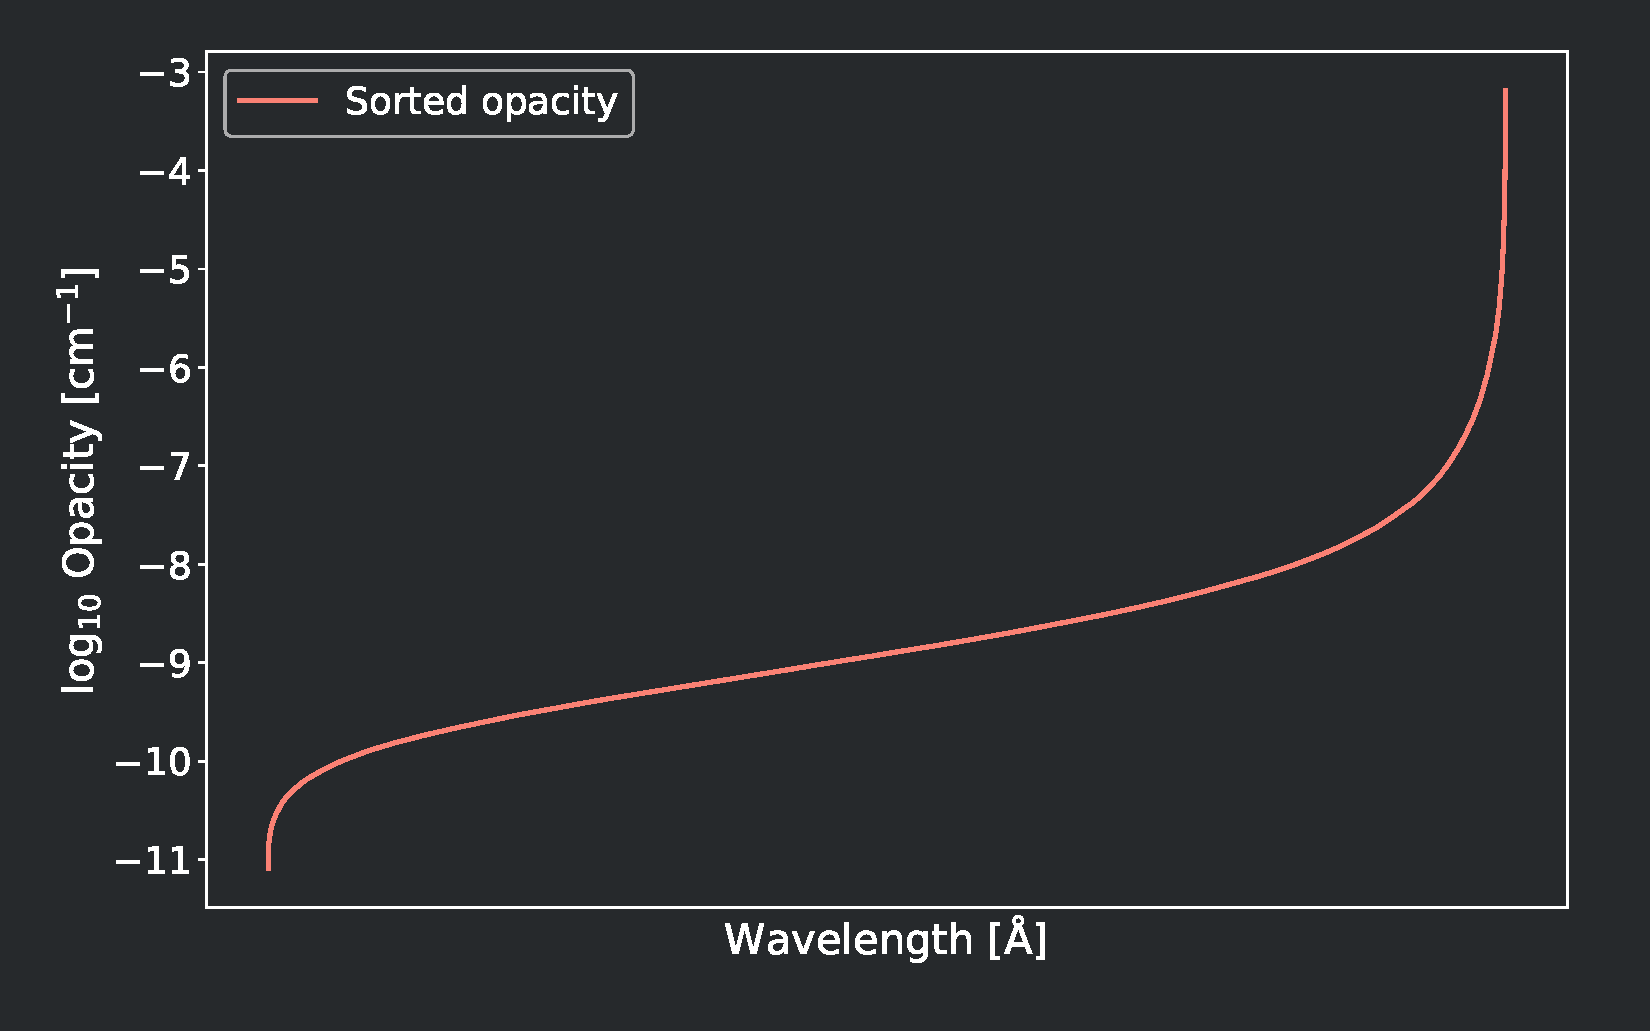
\includegraphics[width=115mm]{images/sorted_opacity_and_sub_bins_0}
}

\frame
{
%...................................................................................................
\note<1>[item]{Take notes here.}
%...................................................................................................
	\frametitle{Approximating the sorted values}
	\begin{itemize}
		\item Approximate opacity with a stepwise function
	\end{itemize}
    \centering
	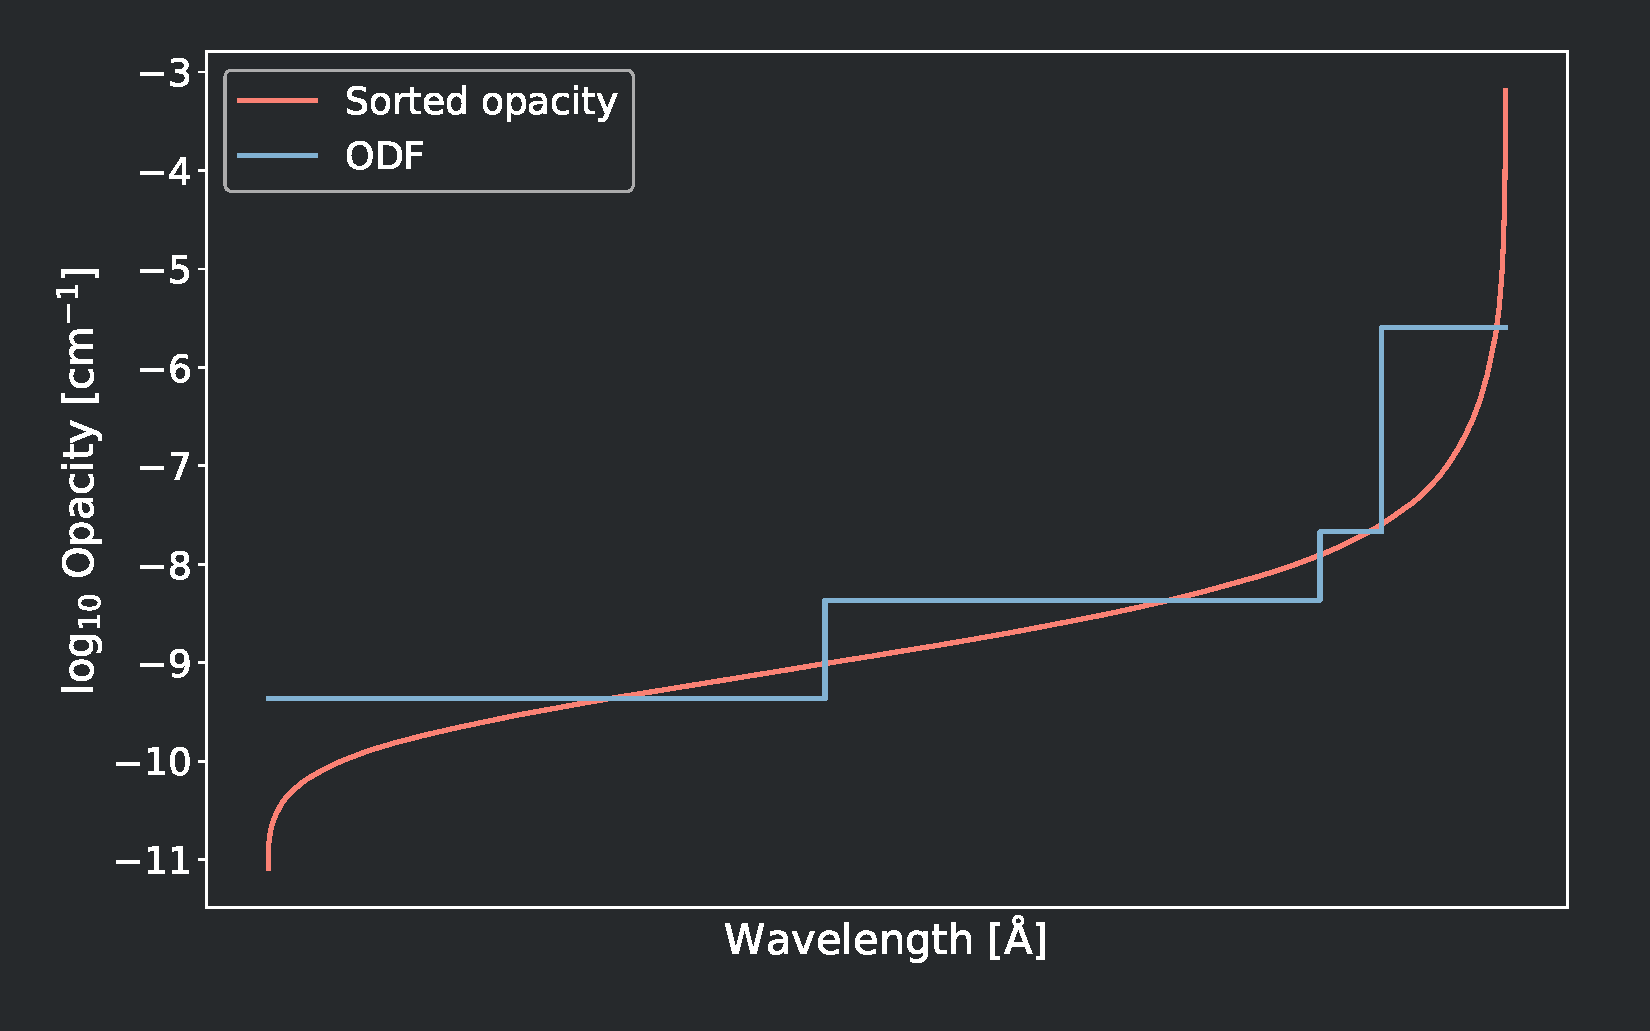
\includegraphics[width=115mm]{images/sorted_opacity_and_sub_bins_1}
}

\frame
{
%...................................................................................................
\note<1>[item]{Take notes here.}
%...................................................................................................
	\frametitle{High resolution spectrum and ODF spectrum}
	\begin{itemize}[(I)]
		\item<1-> Use the stepwise opacity to calculate the flux 
		\item<2-> 4 sub bins -> This two integrals differ by just \alert{2\%}
	\end{itemize}
	\centering
	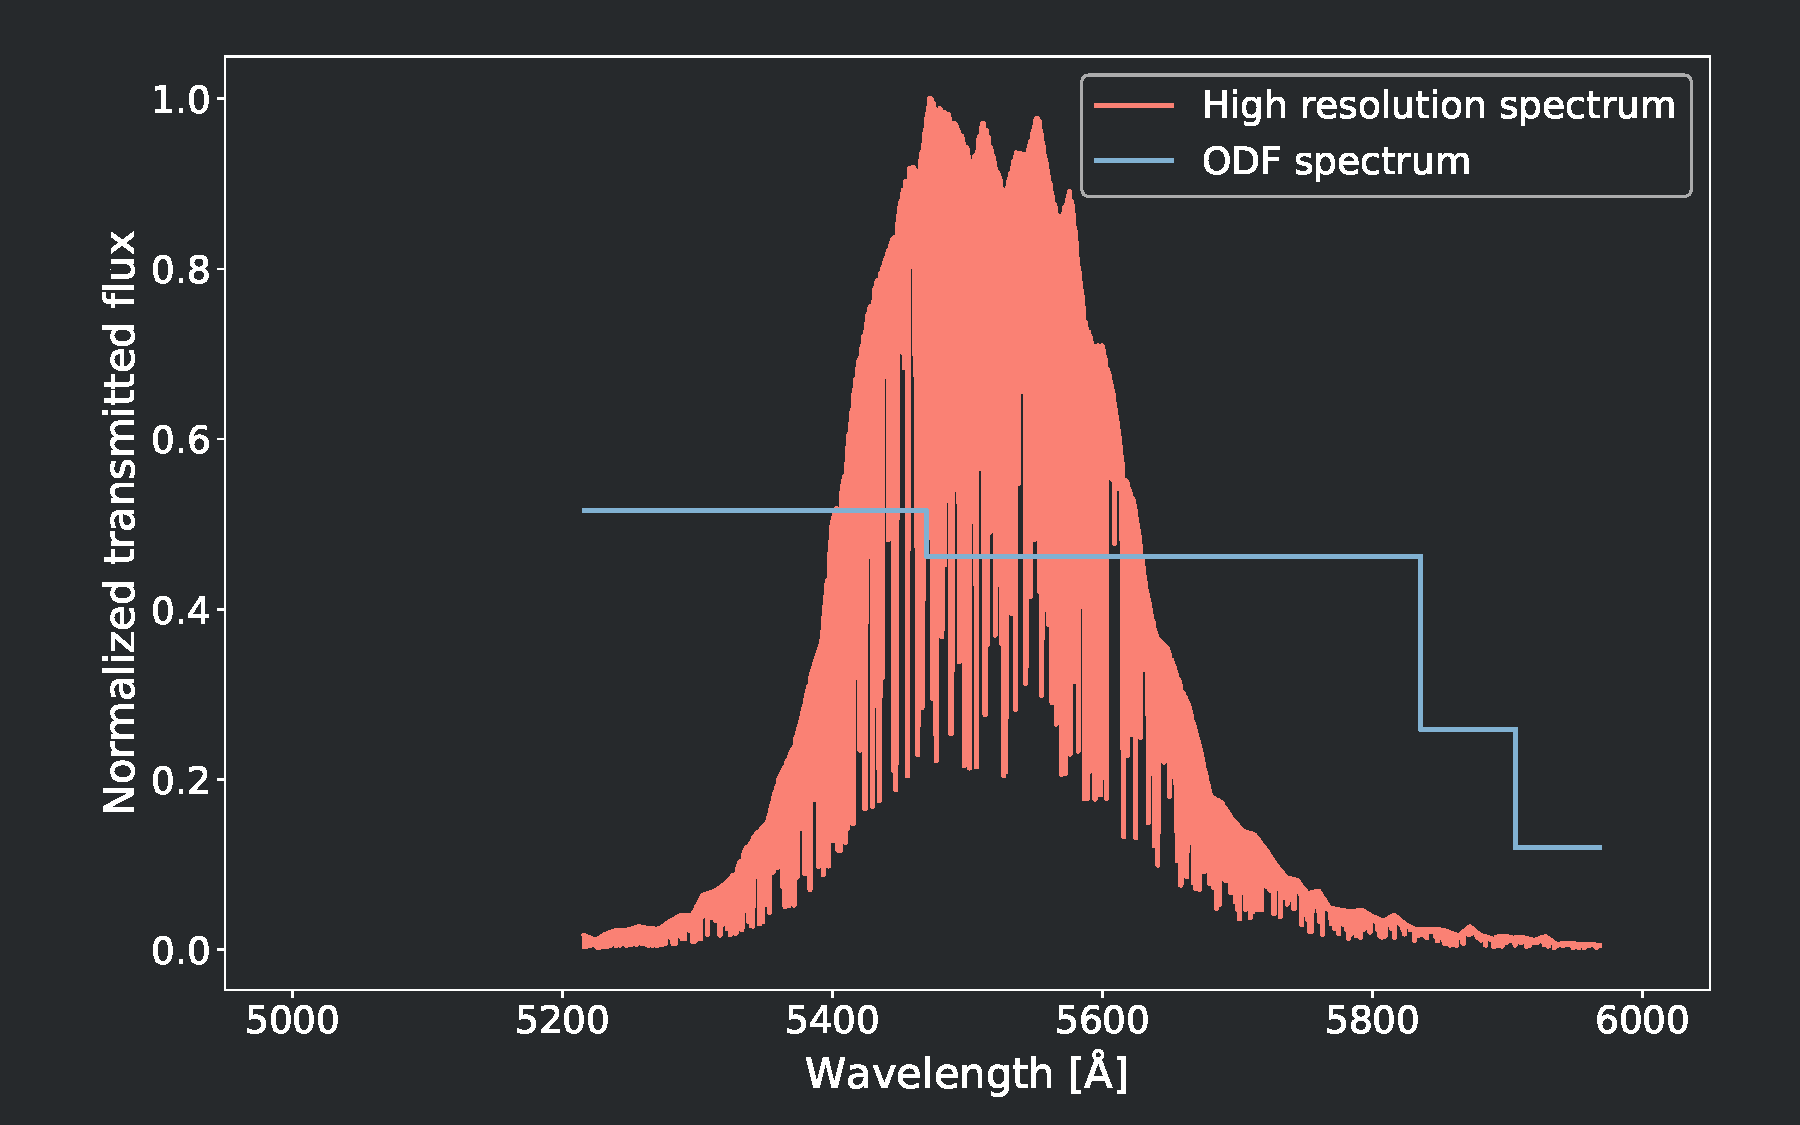
\includegraphics[width=111mm]{images/spectra_transmitted_and_spectra_odf}
}

\frame
{
%...................................................................................................
\note<1>[item]{Take notes here.}
%...................................................................................................
	\frametitle{Generating ODFs}
	\begin{itemize}
    \item Start with high resolution opacity	
	\end{itemize}

	\centering
	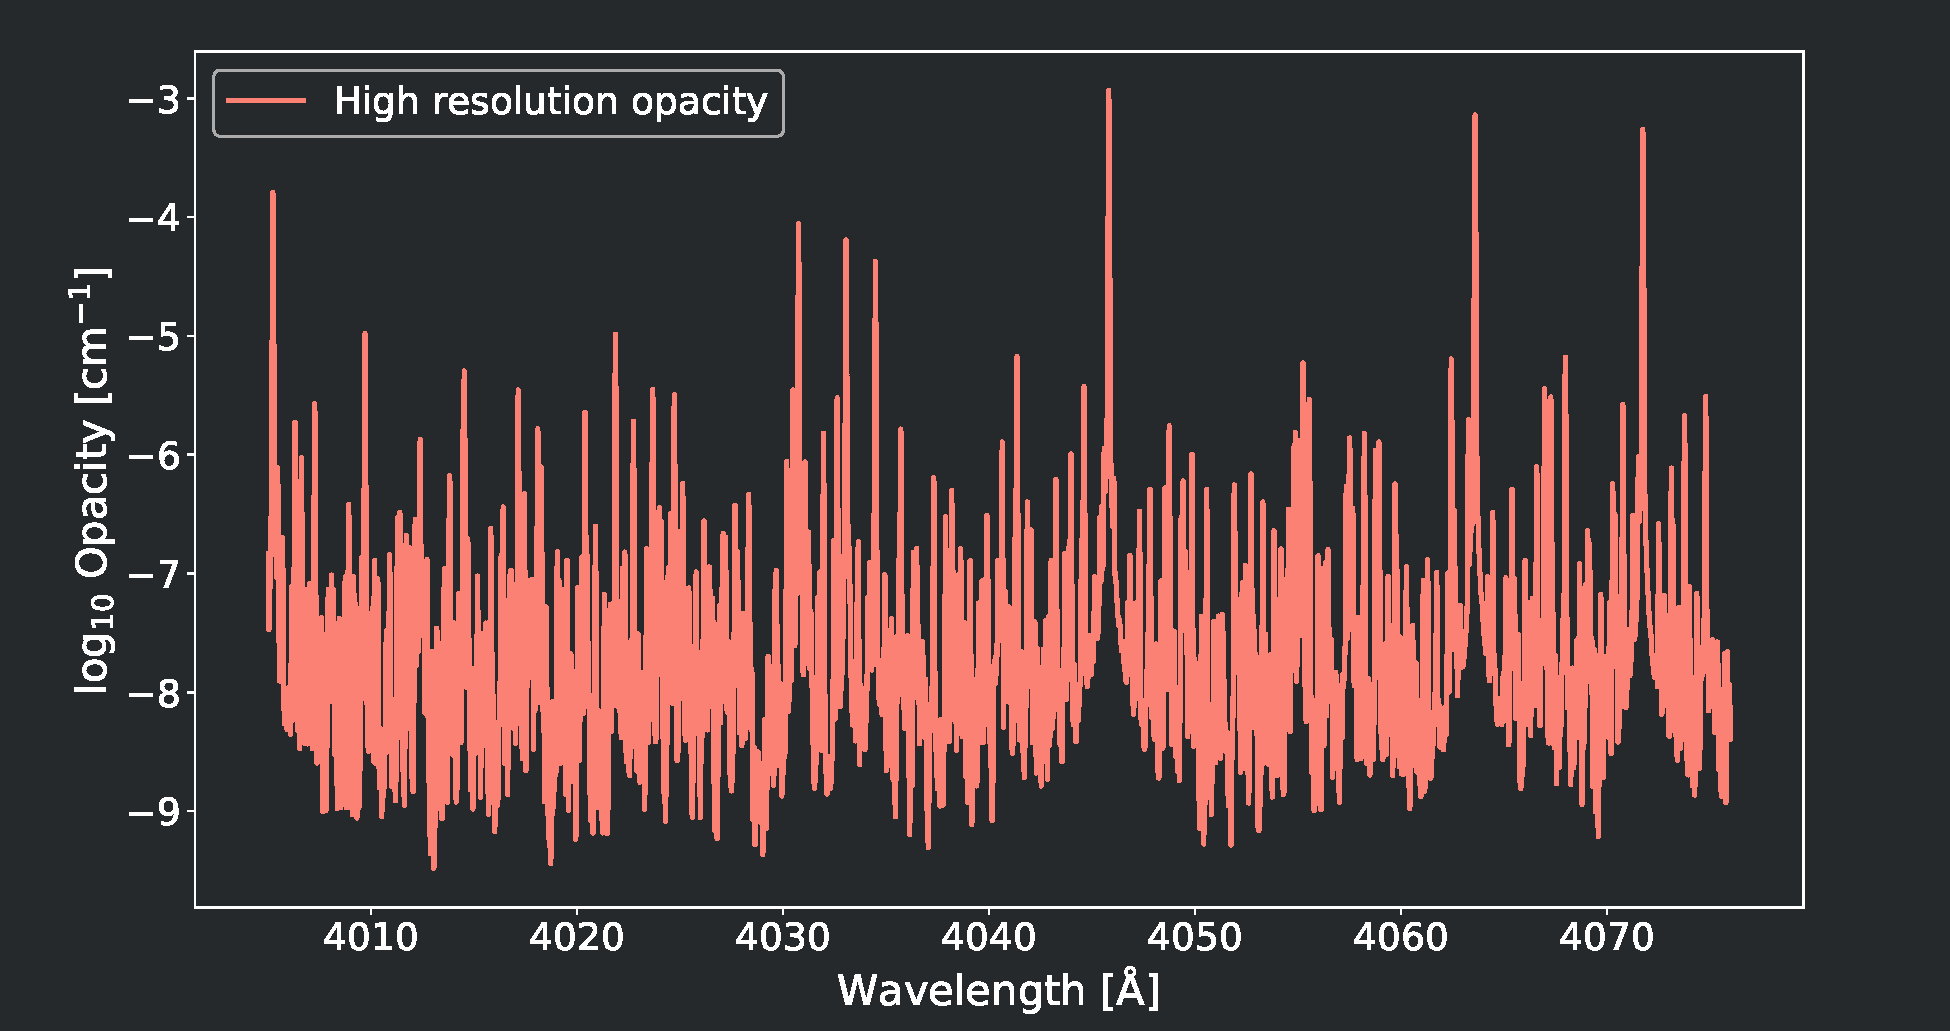
\includegraphics[width=115mm]{images/odf_generation_process_0}
}

\frame
{
%...................................................................................................
\note<1>[item]{Take notes here.}
%...................................................................................................
	\frametitle{Generating ODFs}
	\begin{itemize}
    \item Sort wavelength points by corresponding values of opacity; monotonically increasing opacity
    \item Integral is preserved by sorting
	\end{itemize}		
	\centering
	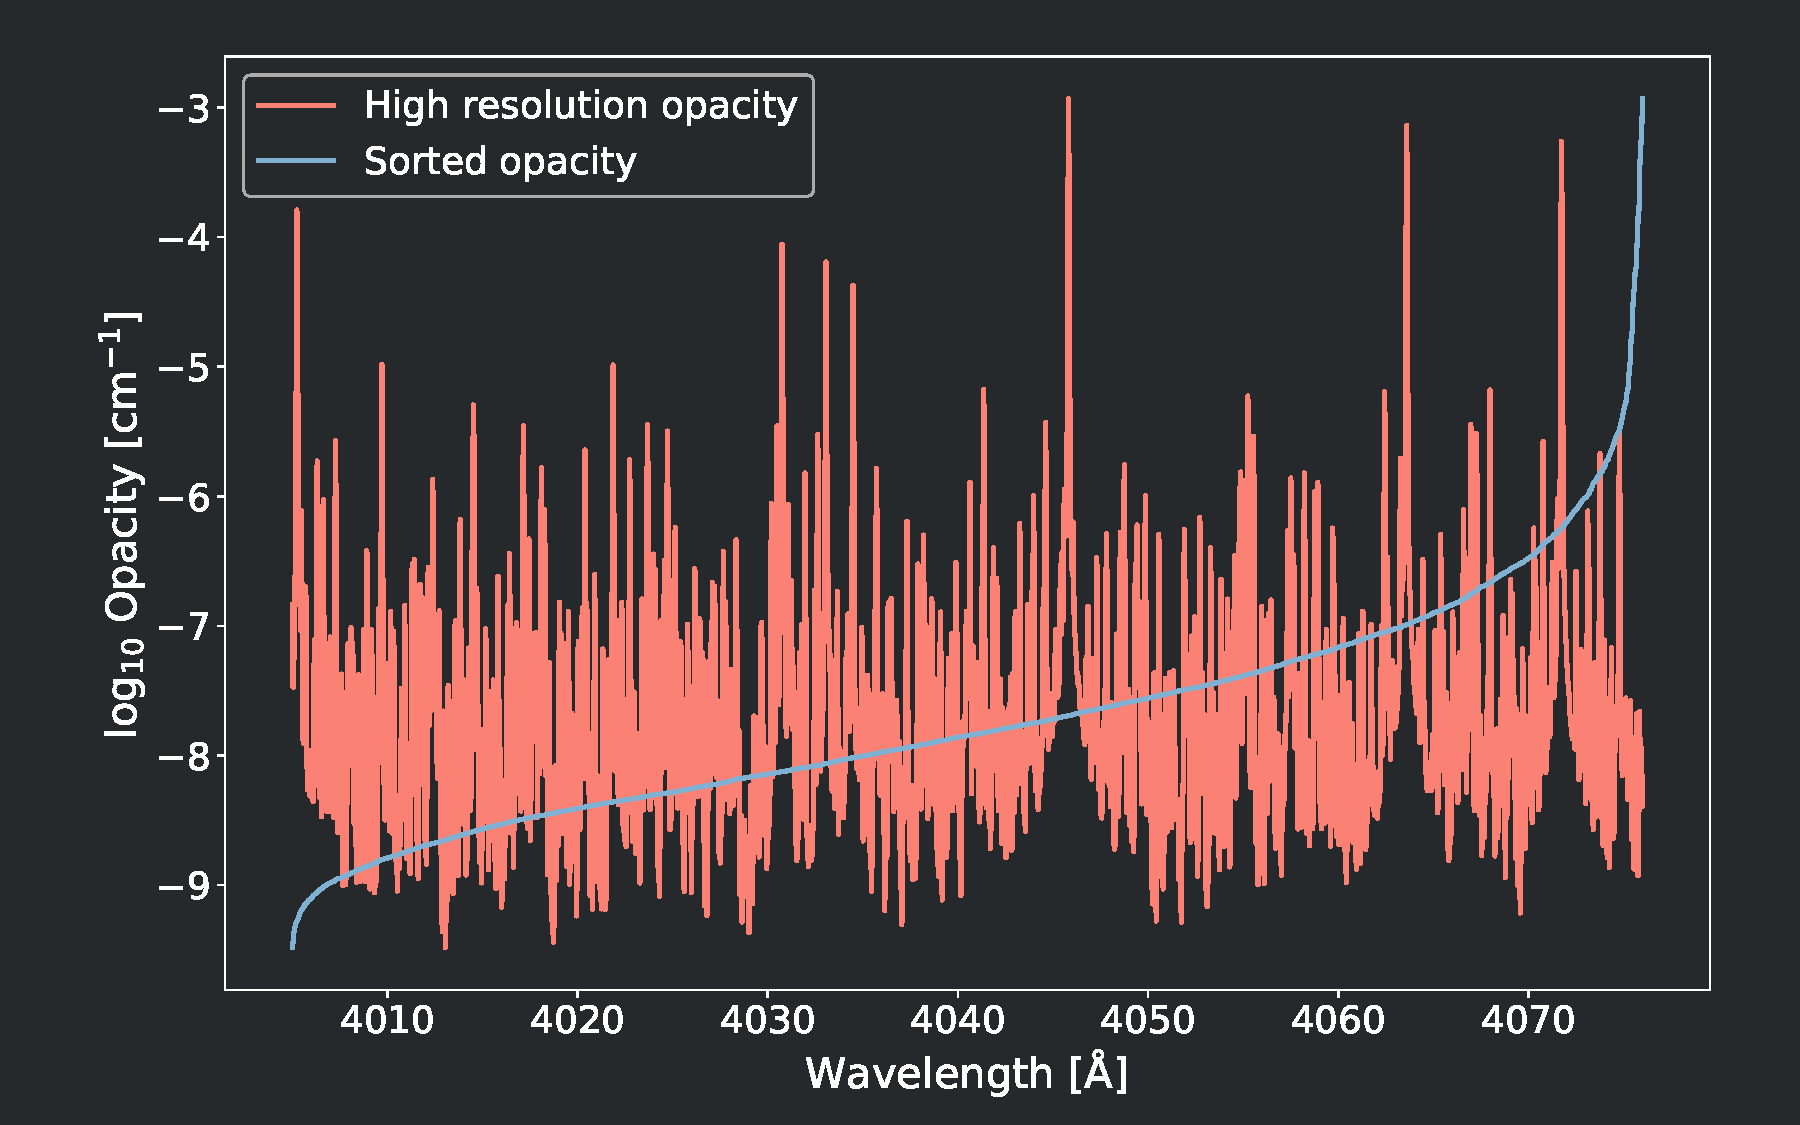
\includegraphics[width=108mm]{images/odf_generation_process_1}
}

\frame
{
%...................................................................................................
\note<1>[item]{Take notes here.}
%...................................................................................................
	\frametitle{Generating ODFs}
	\begin{itemize}
		\item All wavelength information within the bin is lost
\end{itemize}		

		\centering
	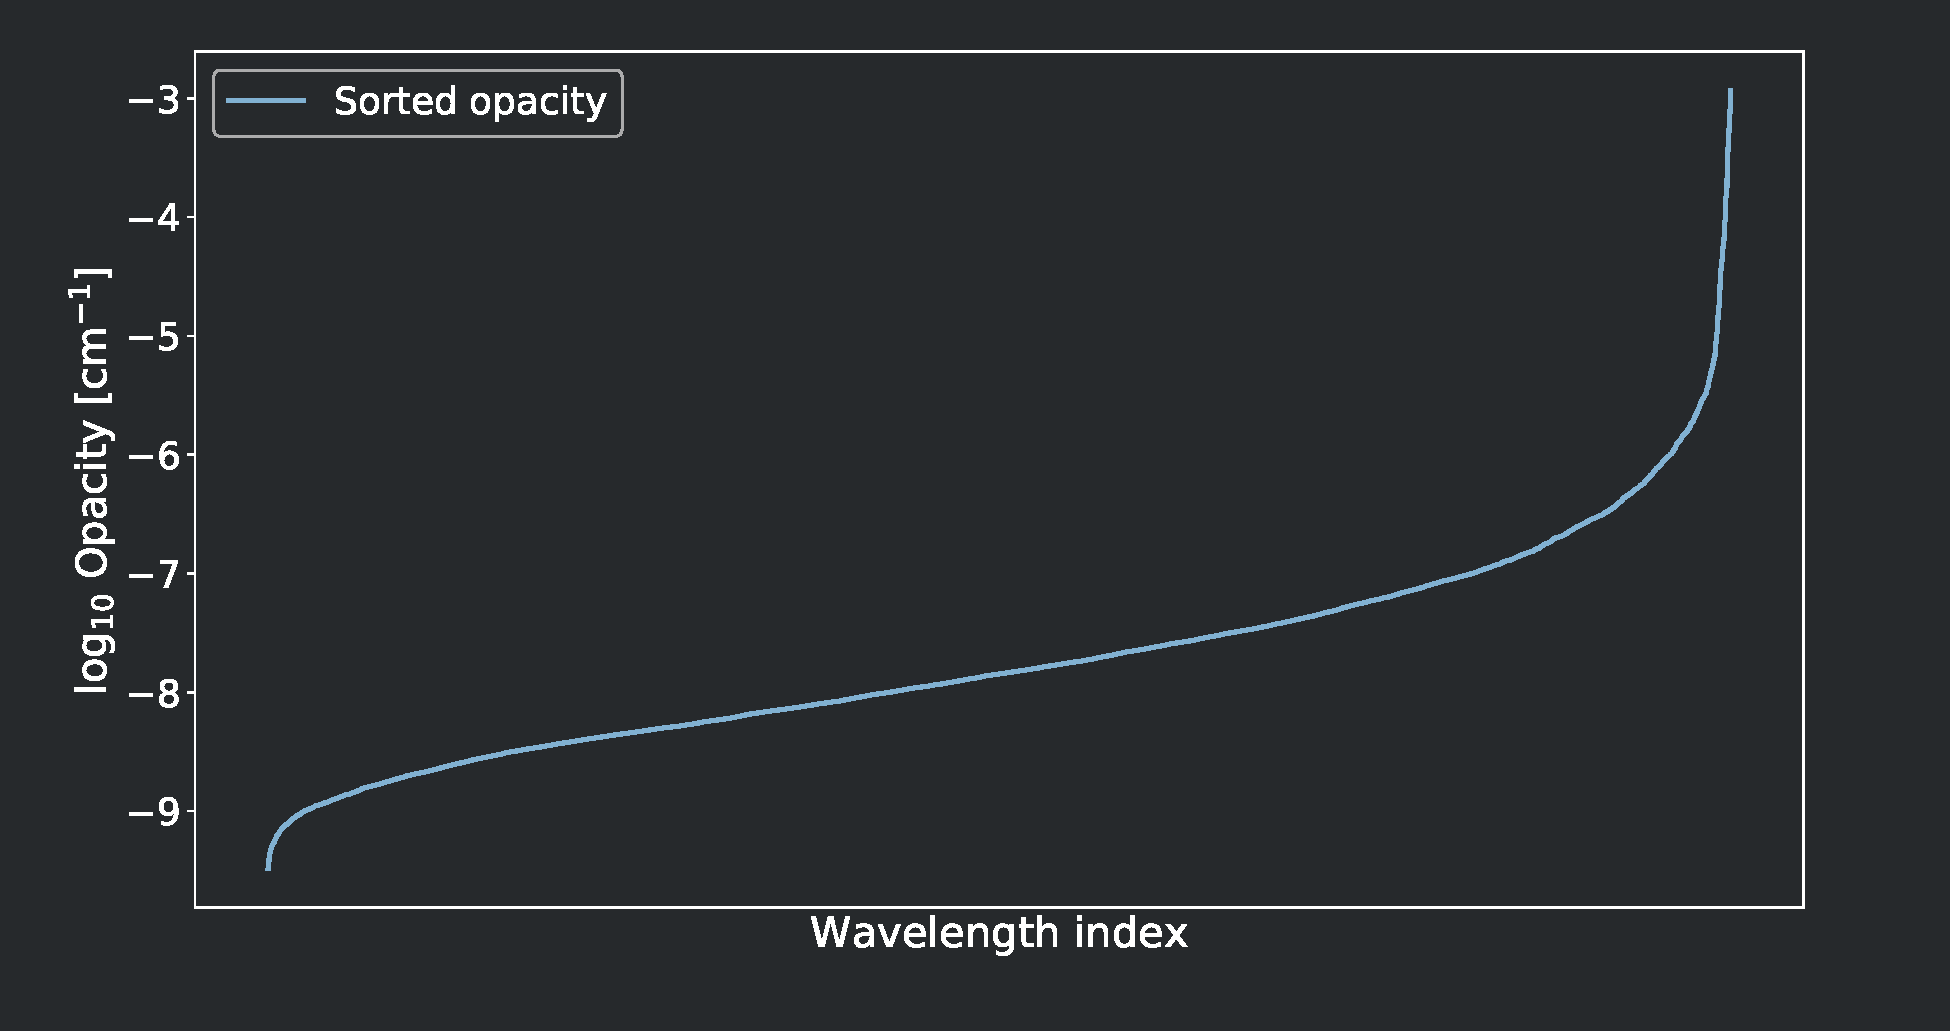
\includegraphics[width=115mm]{images/odf_generation_process_2}
}

\frame
{
%...................................................................................................
\note<1>[item]{Take notes here.}
%...................................................................................................
	\frametitle{Generating ODFs - Example with 10 uniform sub bins}
	\begin{itemize}
		\item Approximate the sorted opacity with a step-wise function
	\end{itemize}
	\centering
	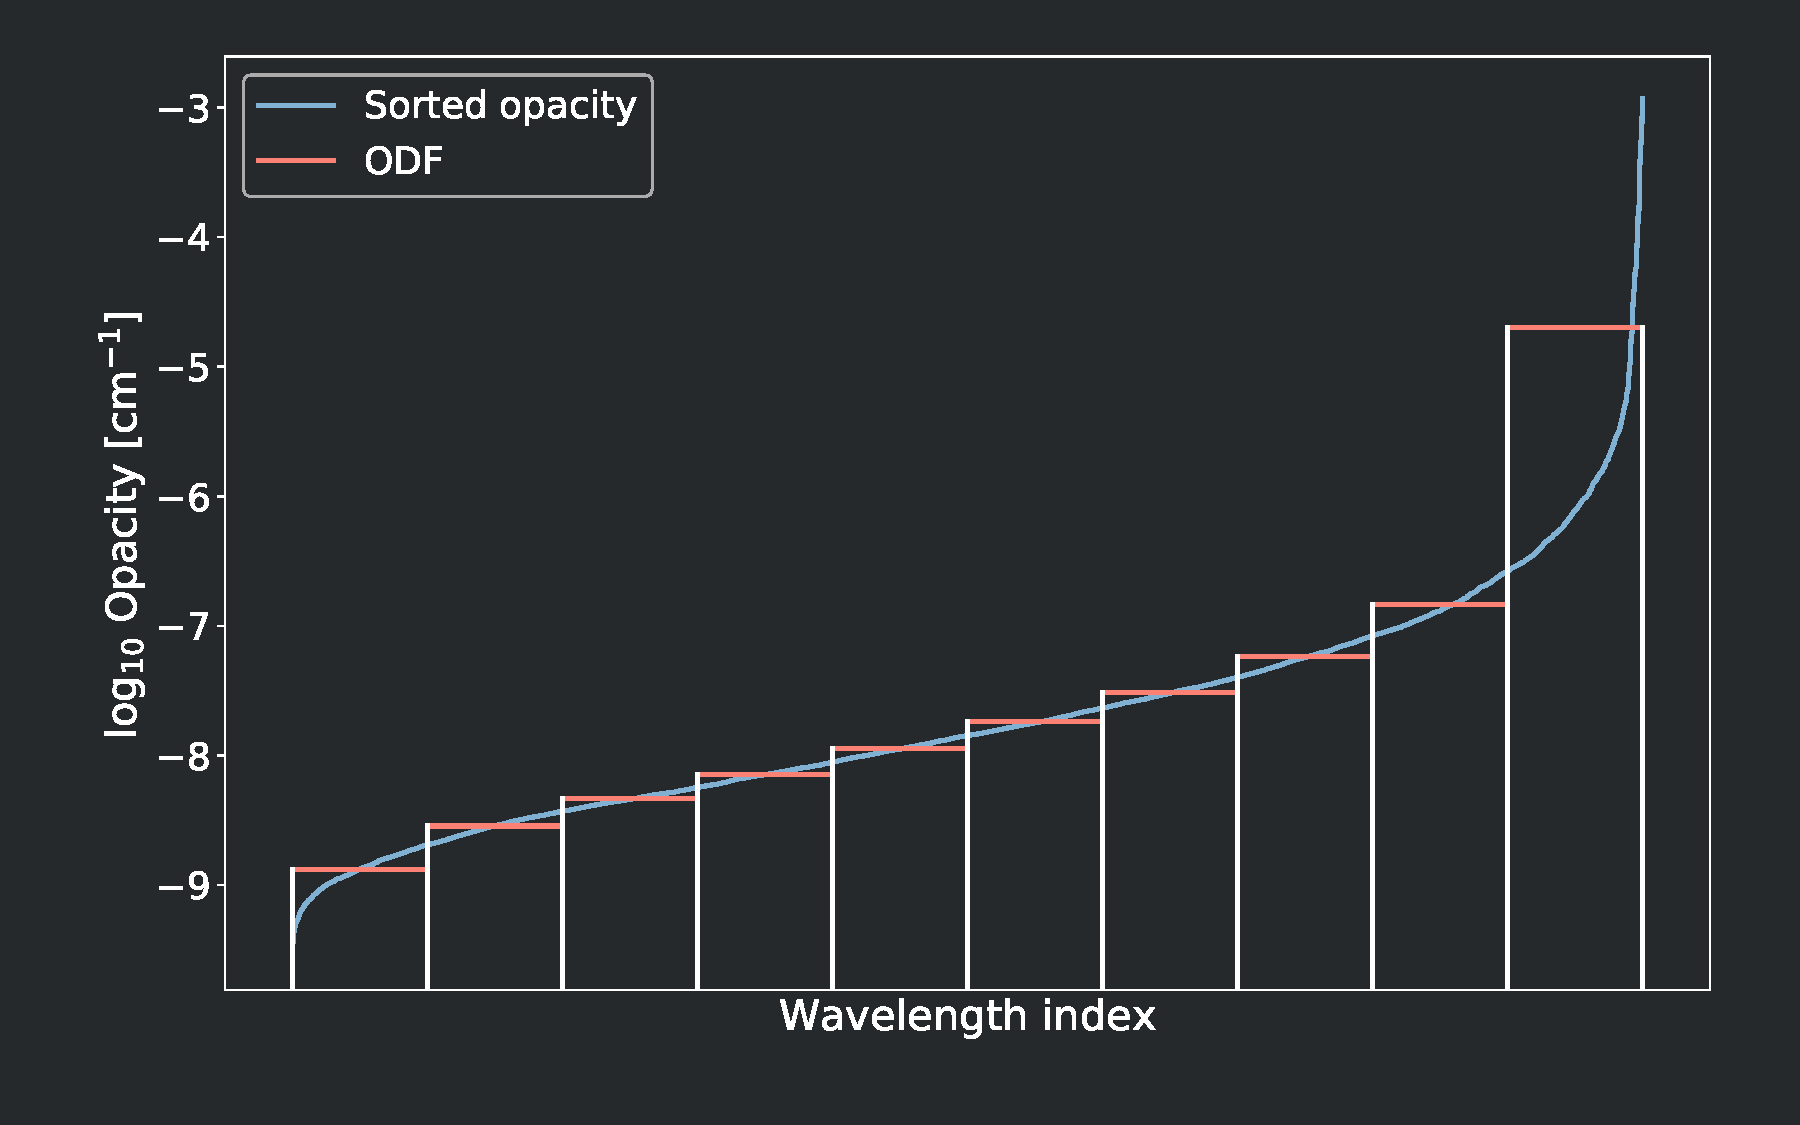
\includegraphics[width=115mm]{images/odf_generation_process_3}
}
\frame
{
%...................................................................................................
\note<1>[item]{Take notes here.}
%...................................................................................................
	\frametitle{ODF generation process}
	\begin{itemize}
	\item Mean is skewed by extreme values
	\end{itemize}
	\centering
	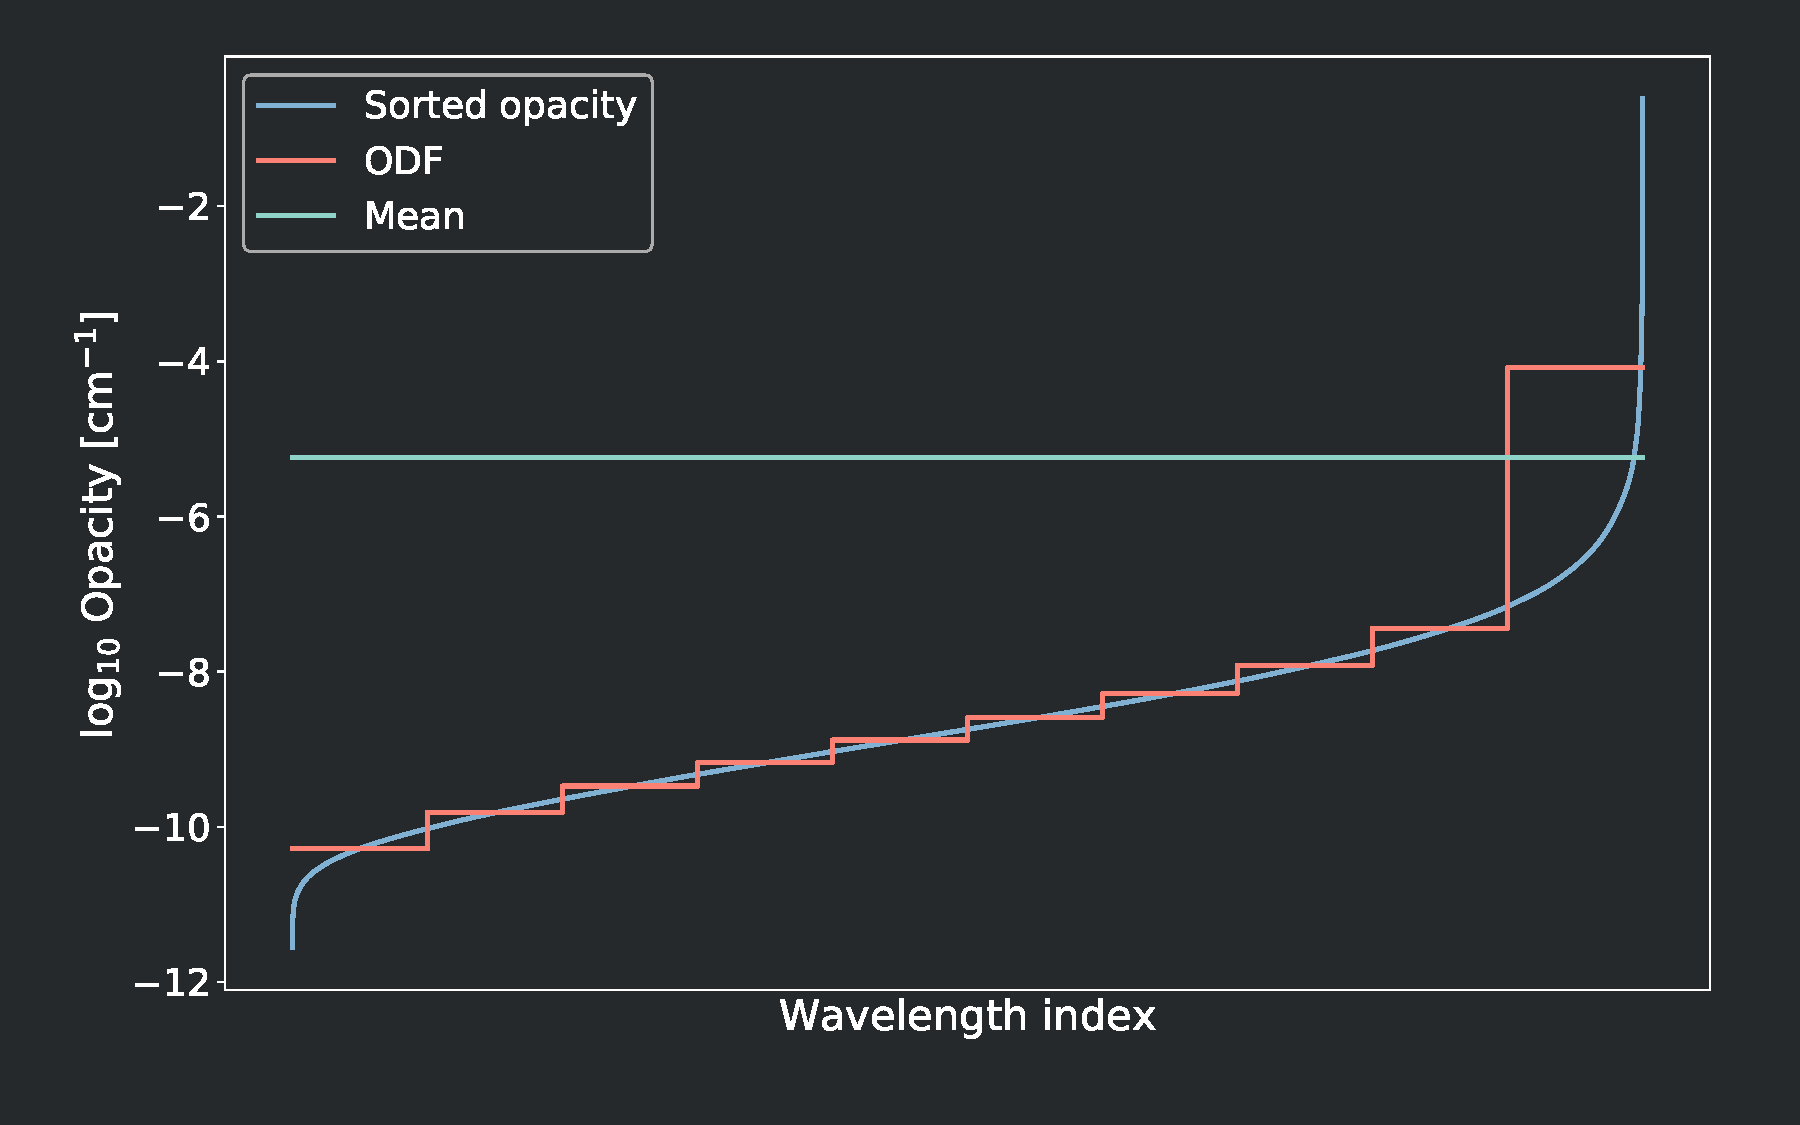
\includegraphics[width=115mm]{images/odf_generation_process_4}
}

\frame
{
%...................................................................................................
\note<1>[item]{Take notes here.}
%...................................................................................................
	\frametitle{ODF performance analysis}
	\begin{itemize}
	    \item Synthesize spectrum using ODFs from 1000-9000\si{\angstrom} with 10\si{\angstrom} bins
	    \item Compare the fluxes from the ODF spectrum with the high resolution spectrum in the bins
	\end{itemize}
	\centering
	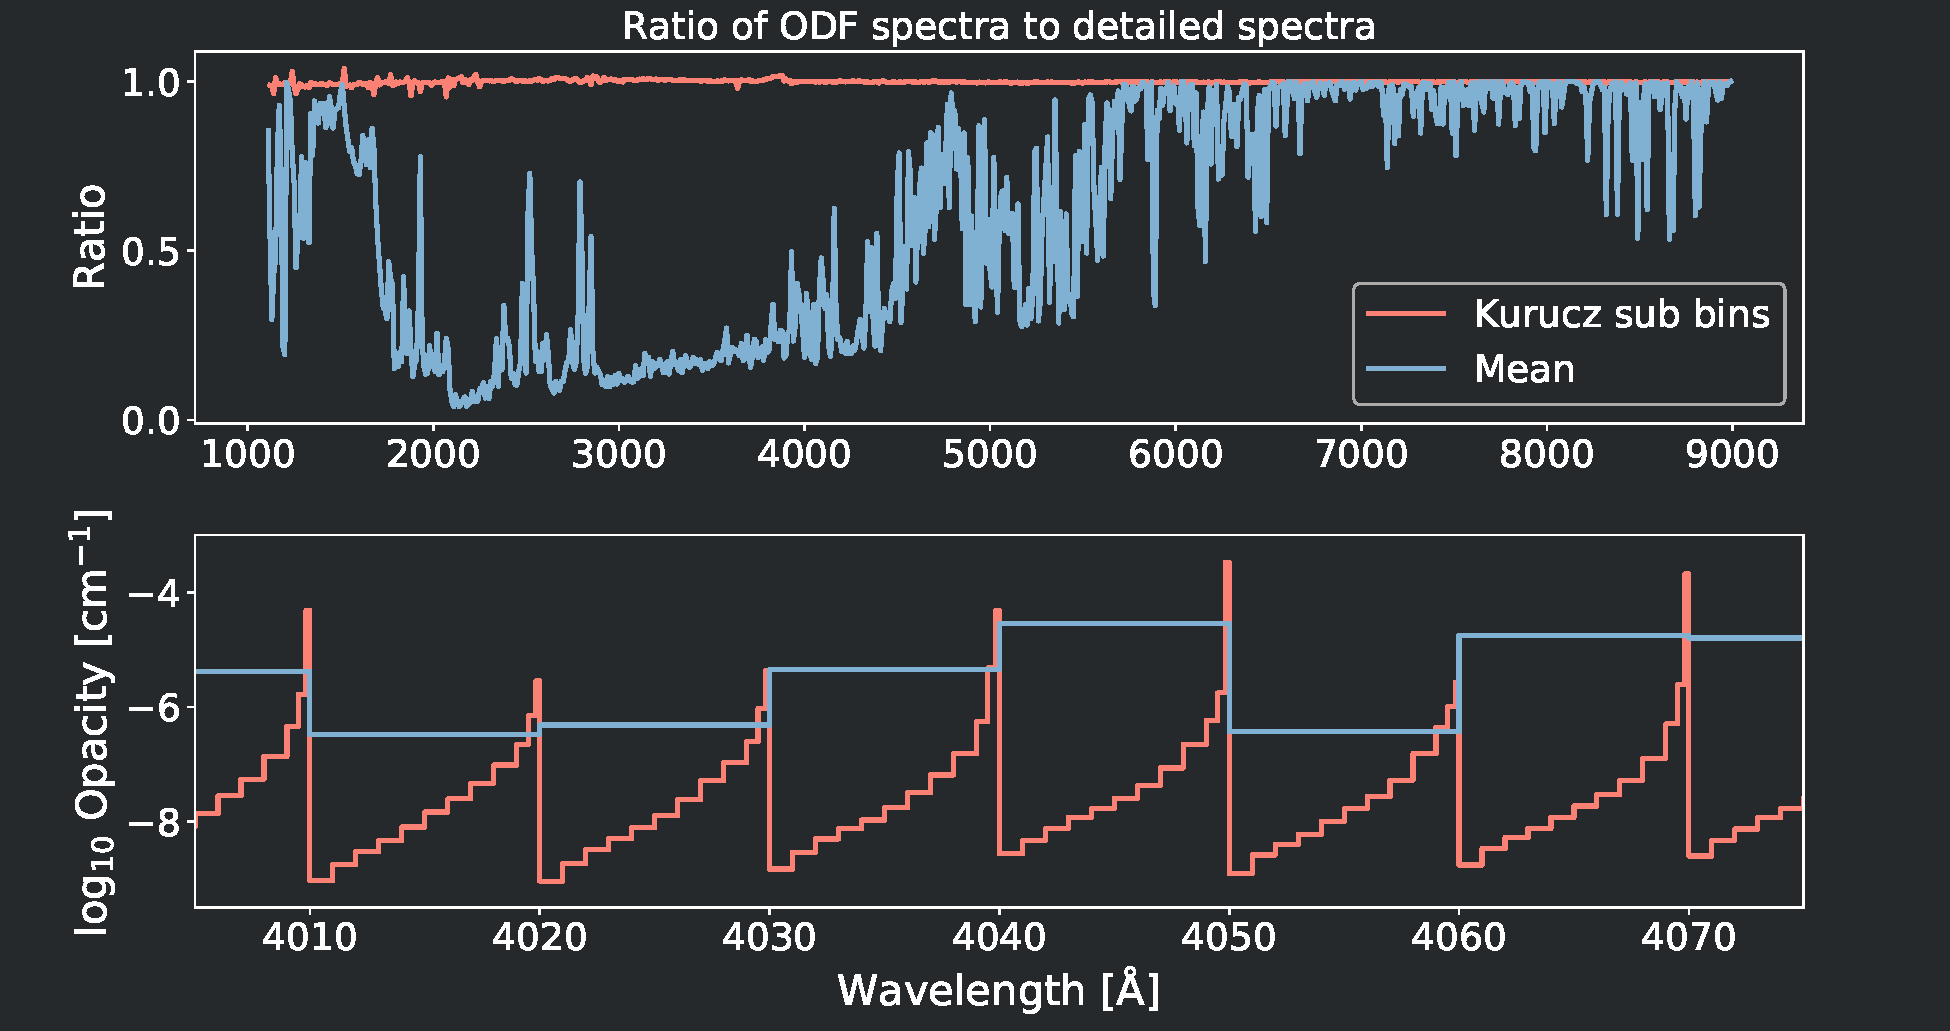
\includegraphics[width=111mm]{images/odf_vs_non_odf}
}

\frame
{
%...................................................................................................
\note<1>[item]{Take notes here.}
%...................................................................................................
	\frametitle{Analysis of different ODFs}
	\begin{itemize}
	\item Uniform ODFs
	\end{itemize}
	
	\centering
	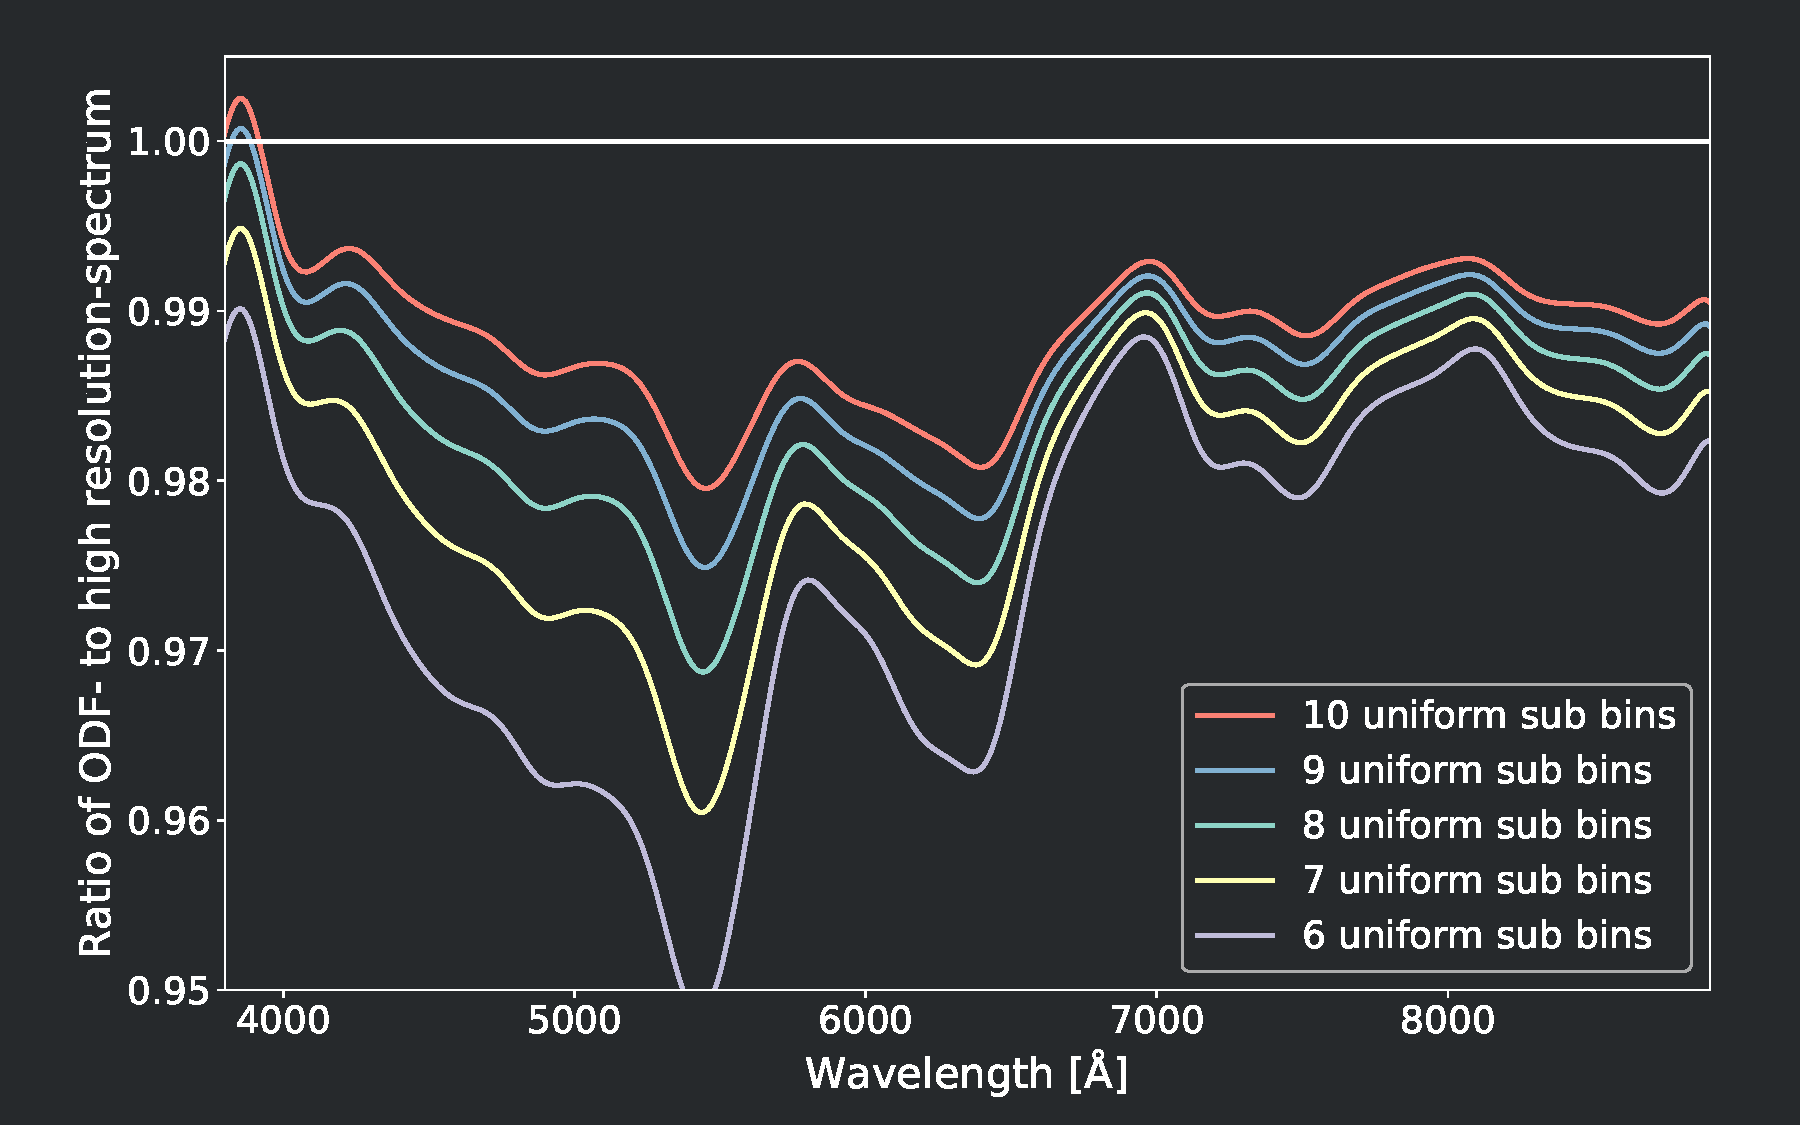
\includegraphics[width=115mm]{images/6_10_vs_best_4_0}
}
\frame
{
%...................................................................................................
\note<1>[item]{Take notes here.}
%...................................................................................................
	\frametitle{Analysis of different ODFs}
	\begin{itemize}
		\item Nonuniform ODFs
		\item The last sub bin is crucial after 5000\si{\angstrom}
    \end{itemize}	  
	\centering
	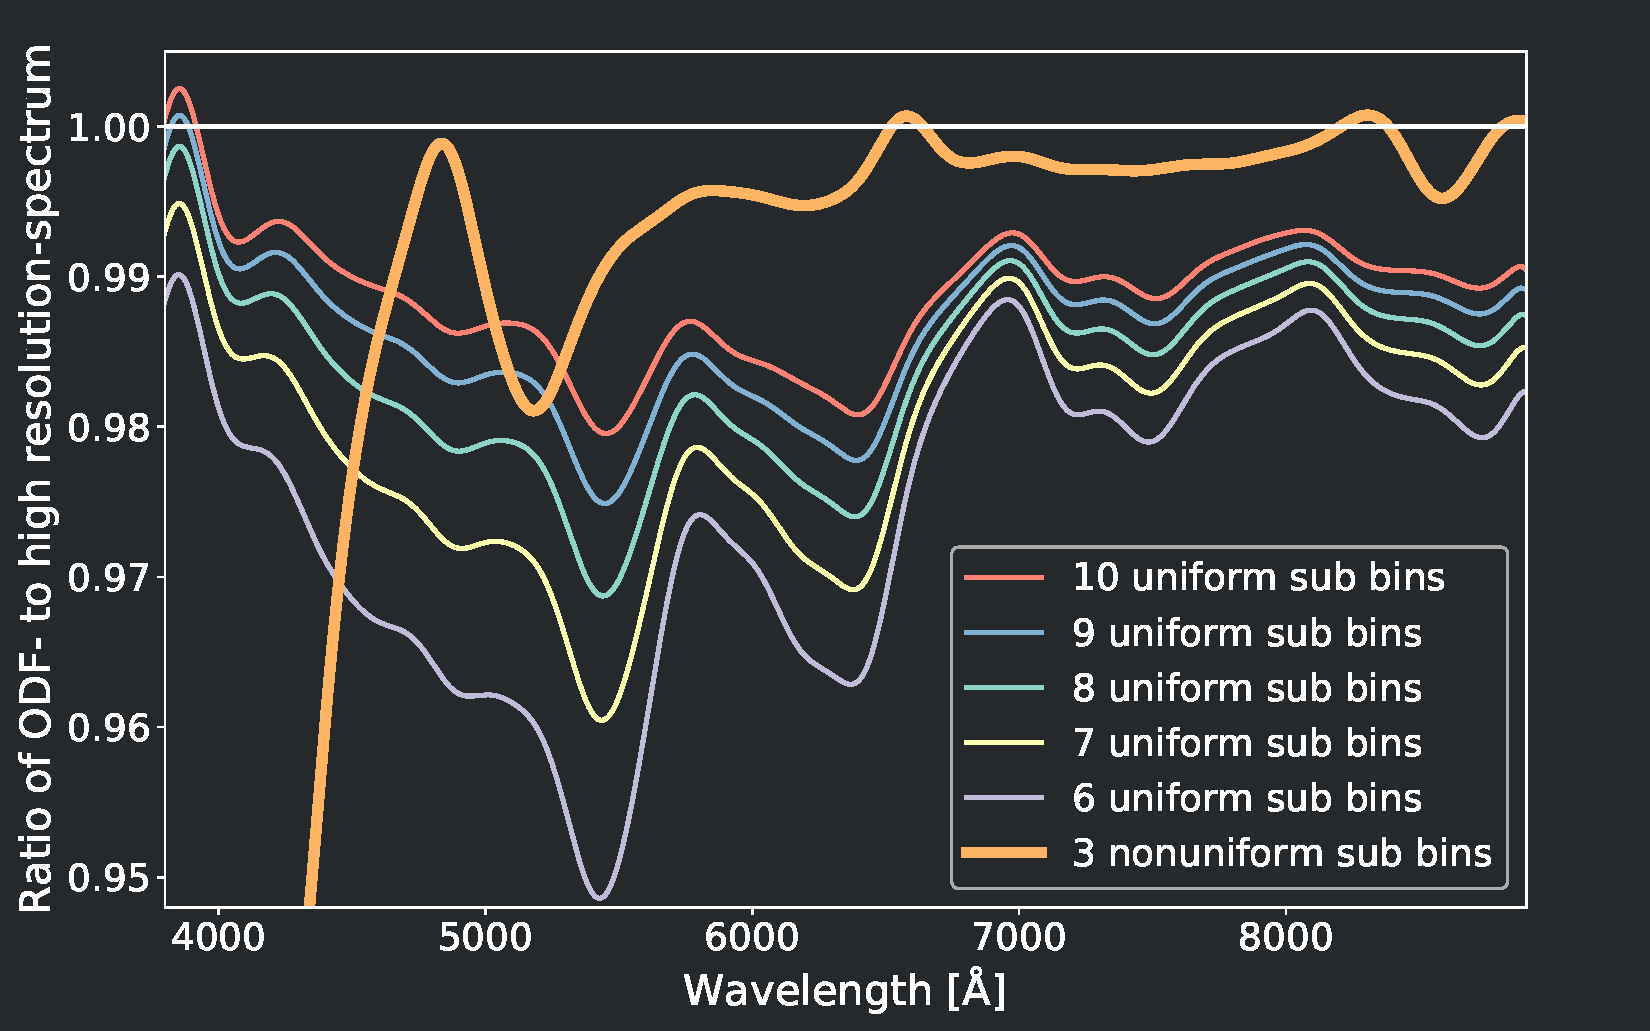
\includegraphics[width=115mm]{images/6_10_vs_best_4_1}
}
\frame
{
%...................................................................................................
\note<1>[item]{Take notes here.}
%...................................................................................................
	\frametitle{Comparison of nonuniform sub bins}
	\begin{itemize}
	    \item Legend specifies sub bin sizes, starting with the first one
	    \item Last sub bin is the same for all
	\end{itemize}
	\centering
	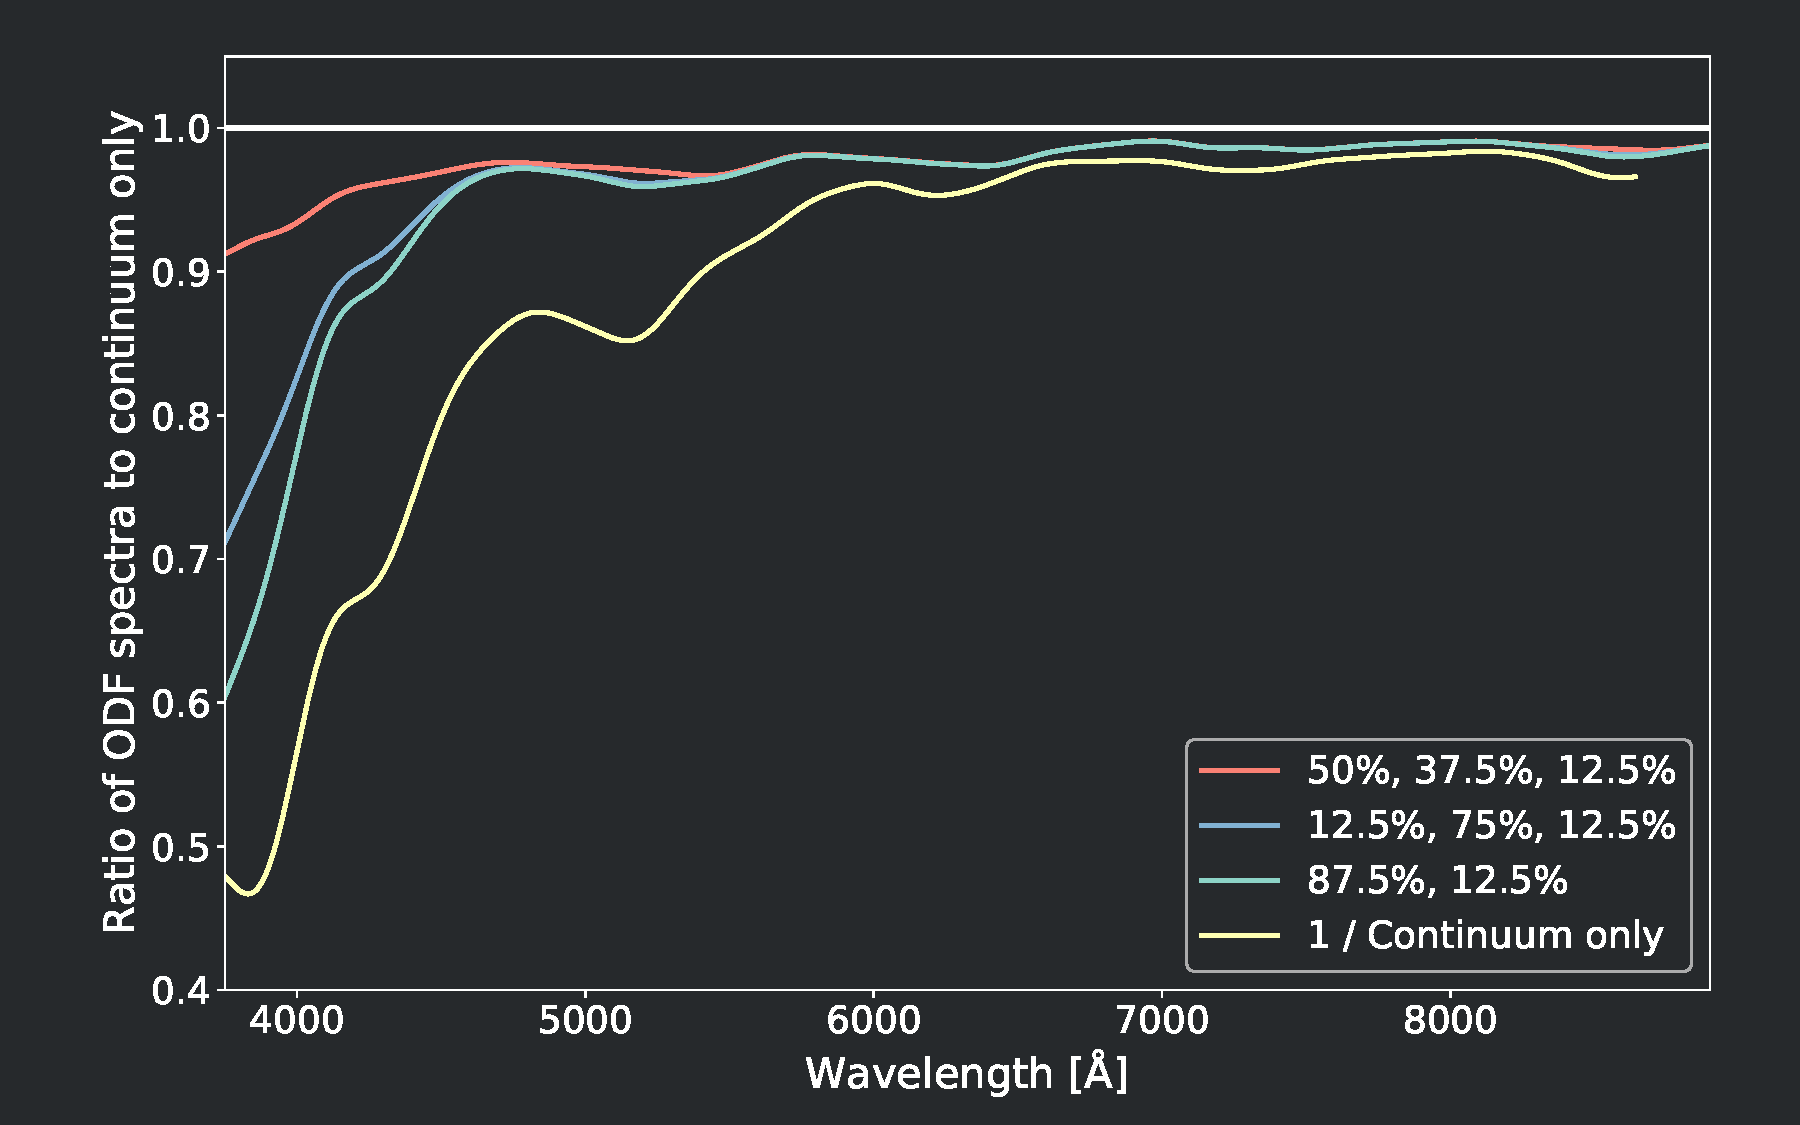
\includegraphics[width=111mm]{images/same_last_sub_bin}
}
\frame
{
%...................................................................................................
\note<1>[item]{Take notes here.}
%...................................................................................................
	\frametitle{Best sub bin combinations using 3 sub bins}
	\centering
	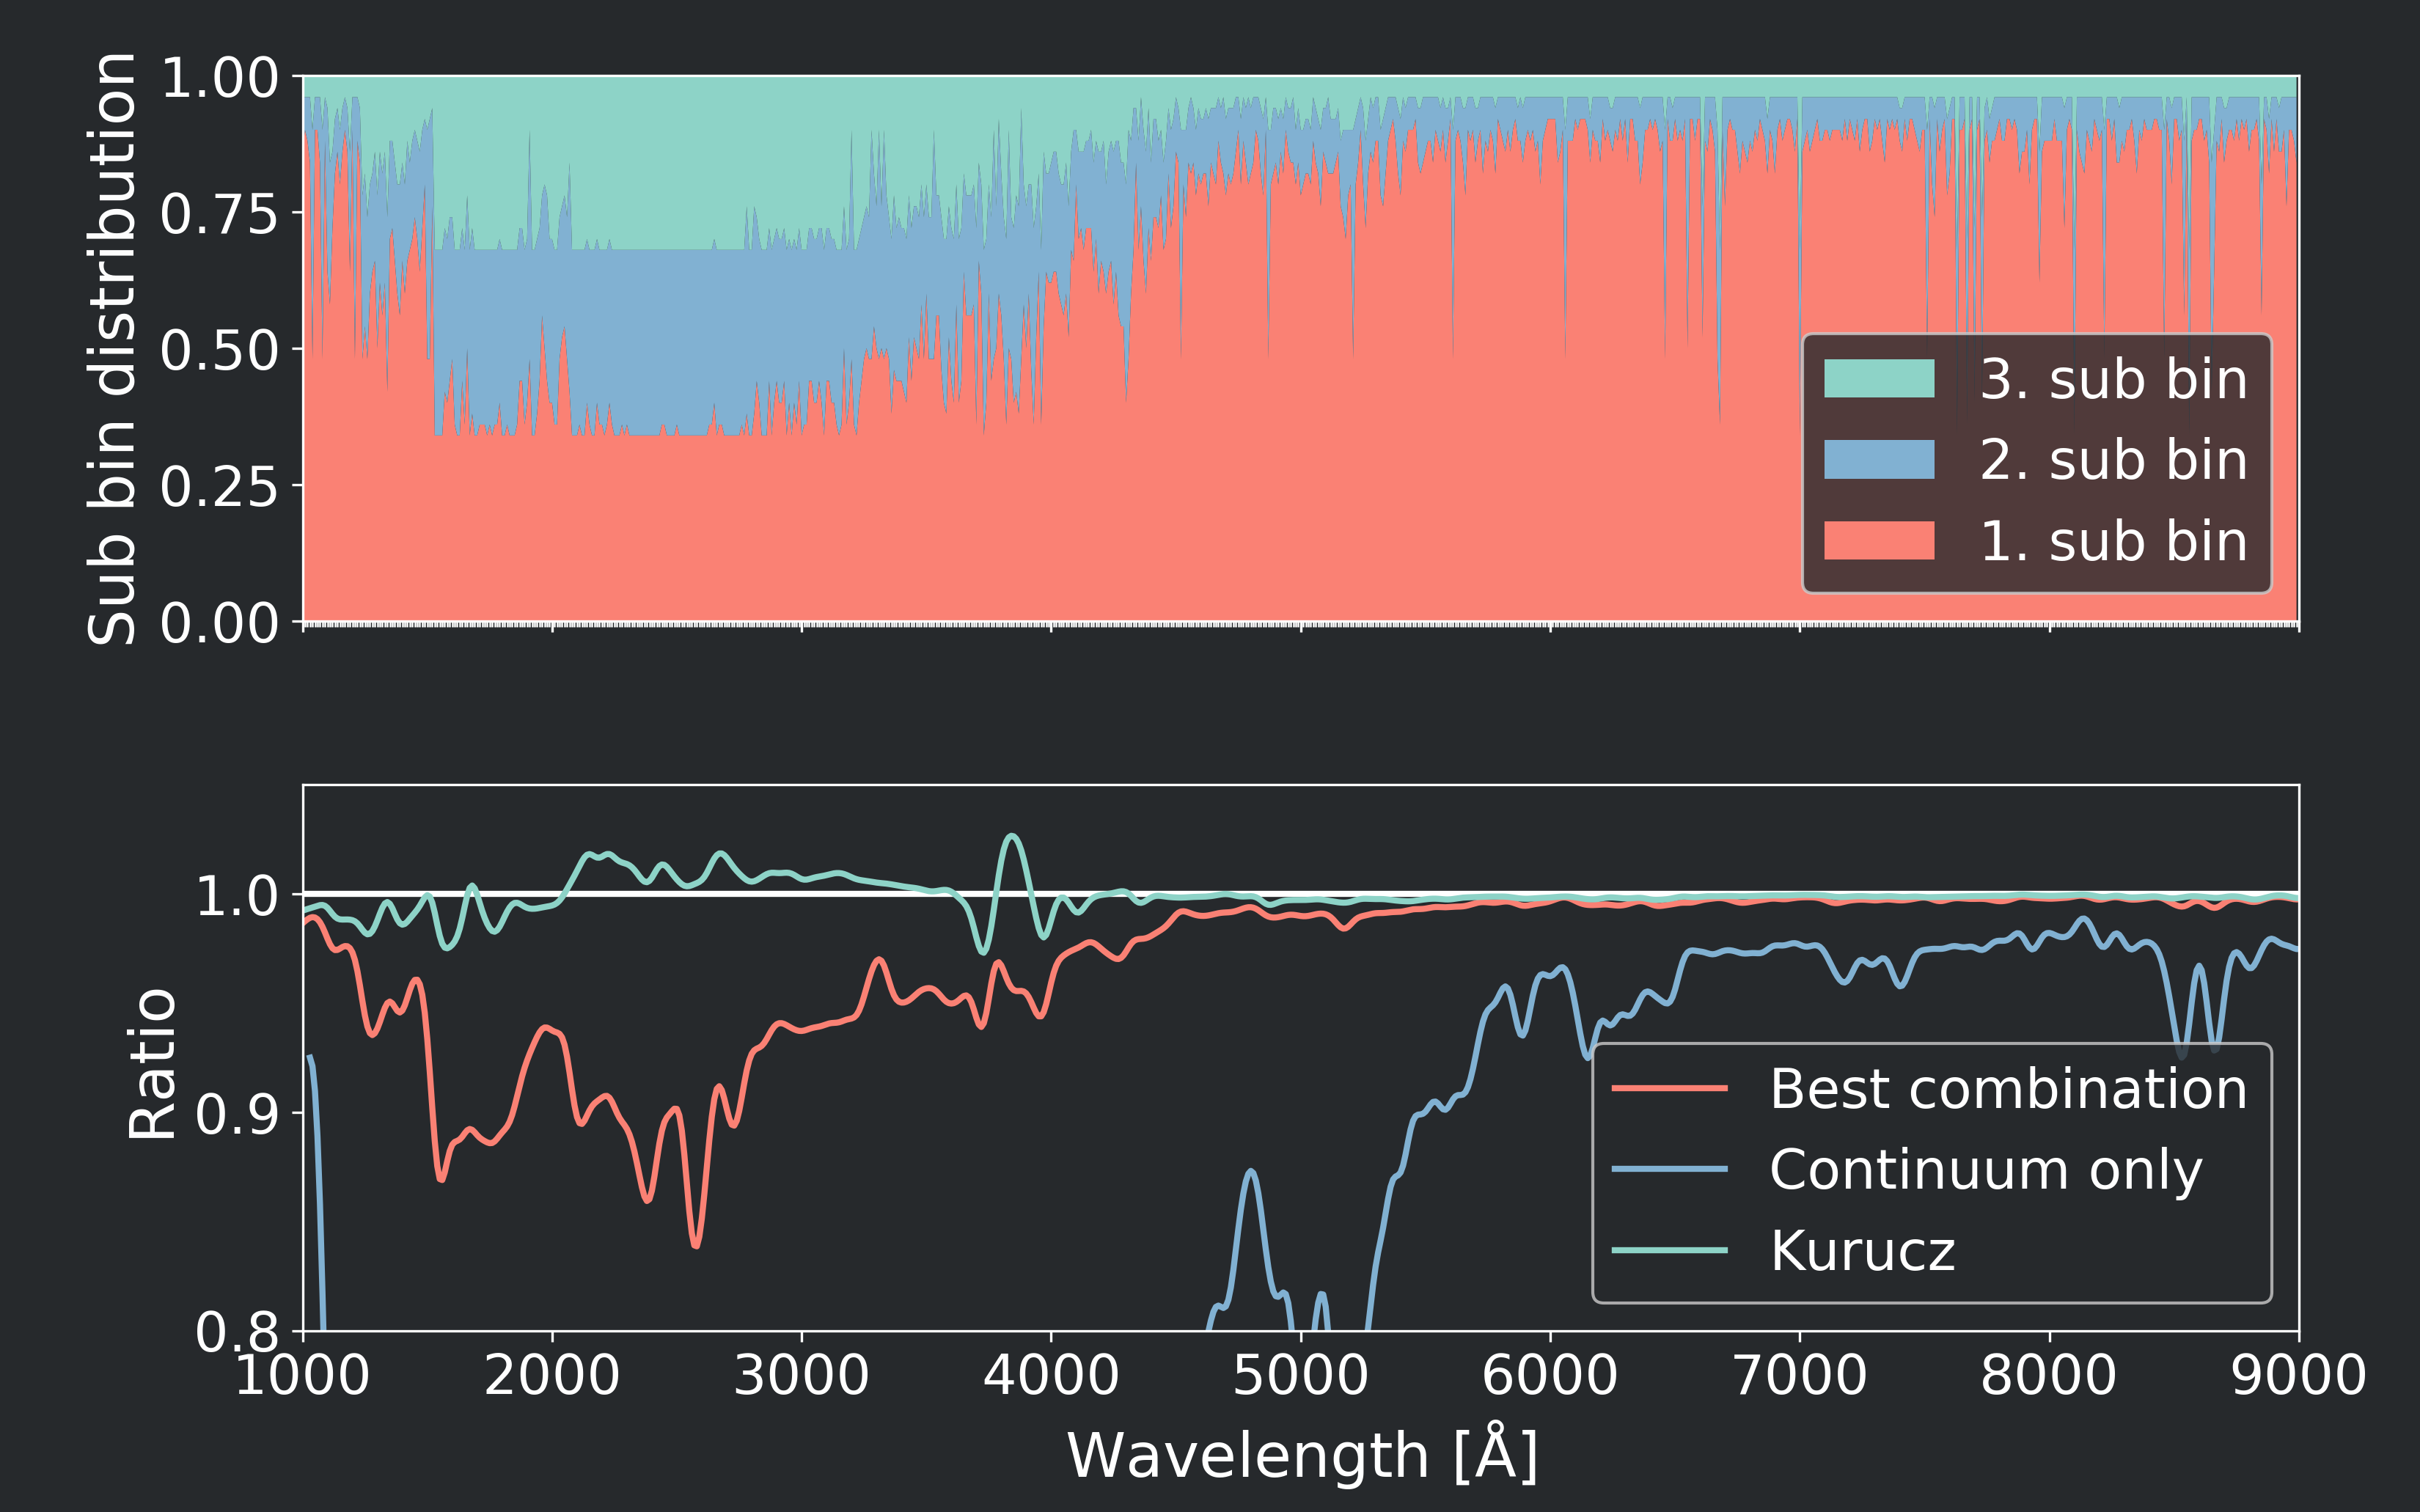
\includegraphics[width=115mm]{images/best_combination}
}
\frame
{
%...................................................................................................
\note<1>[item]{Take notes here.}
%...................................................................................................
	\frametitle{Best combinations of 3 sub bins for Str\"omgren \textit{y}}
	\centering
	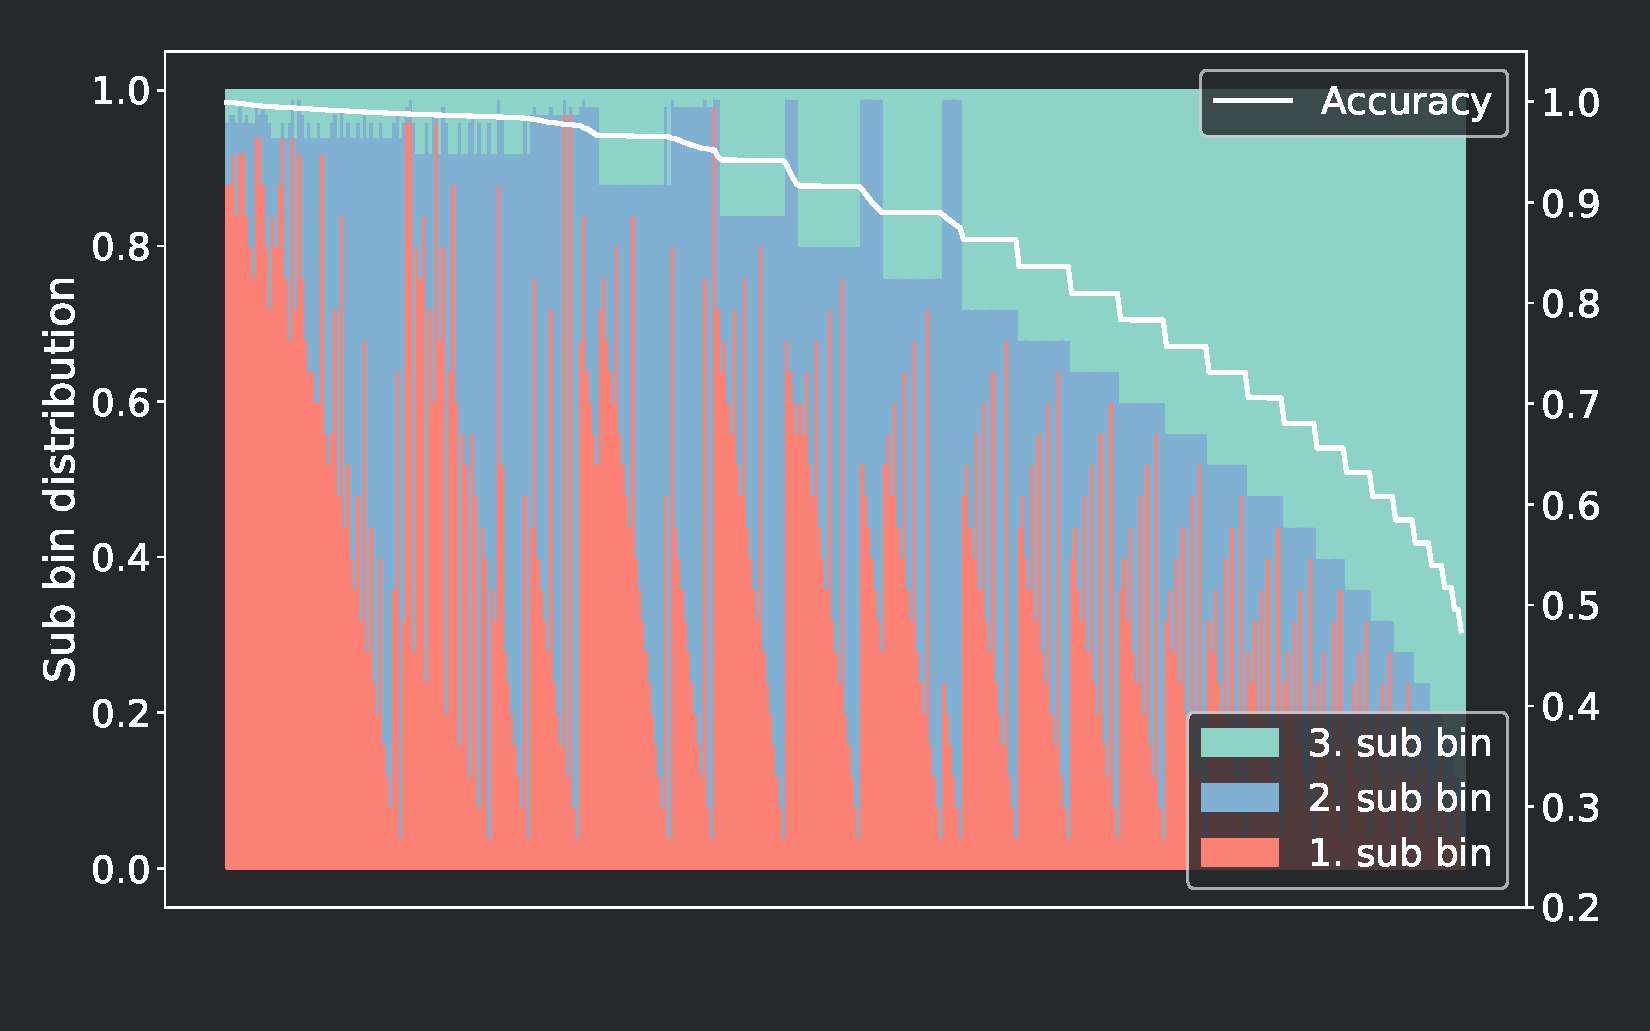
\includegraphics[width=115mm]{images/optimal_stroemgren_0}
}
\frame
{
%...................................................................................................
\note<1>[item]{Take notes here.}
%...................................................................................................
	\frametitle{Best combination of 3 sub bins for Str\"omgren y}
	\centering
	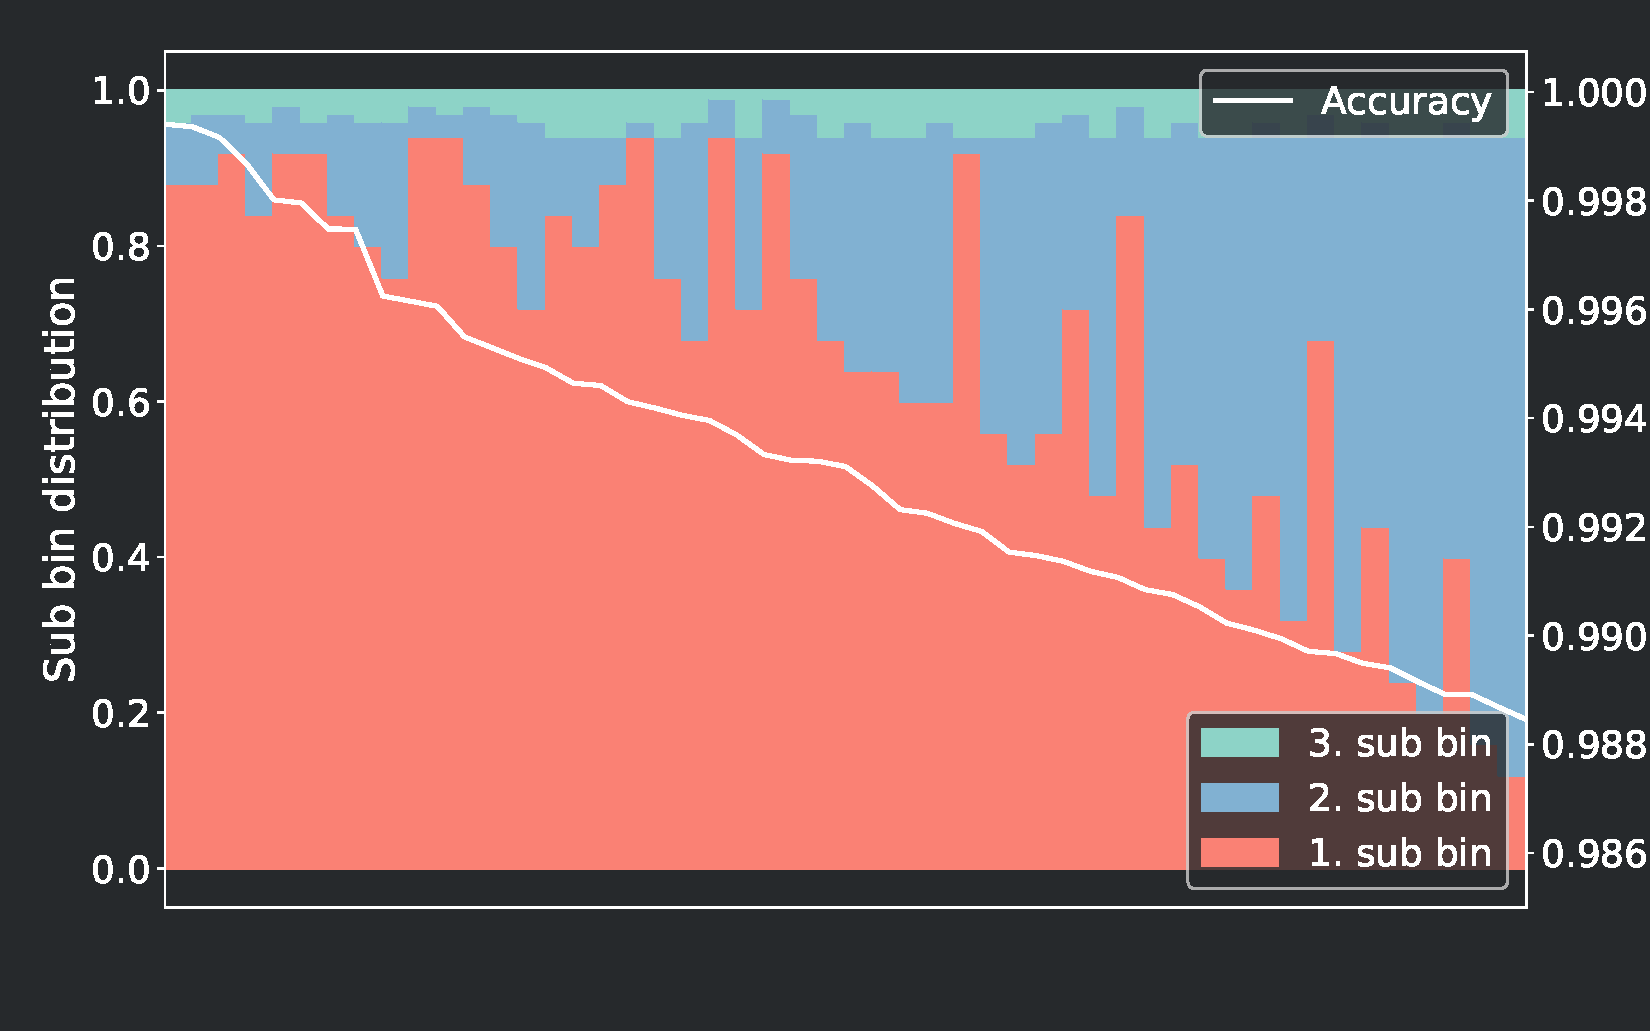
\includegraphics[width=115mm]{images/optimal_stroemgren_1}
}

\frame
{
%...................................................................................................
\note<1>[item]{Take notes here.}
%...................................................................................................
	\frametitle{Speedups in the case of Str\"oemgren \textit{y}}
	\begin{itemize}
		\item Interval length: $\sim$1000\si{\angstrom}\\[20pt]
	\end{itemize}
	
	\centering
%	High resolution calculation 80 points per \si{\angstrom} $\sim$ 80 000 \\
%	ODF calculations 12 points per 10\si{\angstrom} $\sim$ 1200 \\
%	OODF calculations 3 points per 1000\si{\angstrom} $\sim$ 3 \\

\begin{tikzpicture}[sibling distance=25em,
  every node/.style = {shape=rectangle, rounded corners,
    draw, align=center, color=white!20}]]
  \node {\large{High resolution: 80 points per \si{\angstrom} $\sim$ 80 000 points}\\}
    child { node {ODF: 12 points per 10\si{\angstrom} $\sim$ 1200 points \\
    \alert{\large{speedup 67 times}}} }
    child { node {OODF: 3 points per 1000\si{\angstrom} $\sim$ 3 points \\
    \alert{\large{speedup 25 000 times}}} };
\end{tikzpicture}

}

\frame
{
%...................................................................................................
\note<1>[item]{Take notes here.}
%...................................................................................................
	\frametitle{Conclusions}
	\large{
	\begin{itemize}
	\item An efficient  procedure for radiative transfer is timely for new generation of solar and stellar variability models.\\[15pt]
	\item We developed a novel method for fast spectral synthesis. \\[15pt]
	

    \item Can be tailored for different filters: Strömgren \textit{b} + \textit{y}, Kepler, PLATO  and others.\\[15pt]


    \item Significant speed up relative to standard  methods by a factor of at least two orders of magnitude.\\[10pt]
	\end{itemize}
	
	}
	\pause
	
		\centering \alert{\Large{Thank you for your attention!}}
}
